\documentclass[12pt,oneside,final]{book}




\usepackage[portuges,brazil]{babel}
\usepackage[utf8]{inputenc}


\usepackage{indentfirst}
\usepackage{ae}
\usepackage{natbib}

\usepackage[T1]{fontenc}
\usepackage{lmodern}


\usepackage{amssymb,fancyhdr,fancybox,epsfig,psfrag,tabularx,setspace}
\usepackage{amsmath}
\usepackage[paperwidth=8.5in,paperheight=11in,hmargin={25mm,20mm},vmargin={20mm,20mm}]{geometry} %tamanho letter

\usepackage[chapter]{algorithm}
\usepackage{algorithmic}



\floatname{algorithm}{Algoritmo}

\usepackage{epstopdf}
\DeclareGraphicsExtensions{.pdf,.jpeg,.png,.eps}

\def\tituloTese{} \def\aluno{Isaac Leonardo Santos Sacramento} 
\def\nomeProf{Mauro Roisenberg} 
\def\professor{Prof. Dr. \nomeProf}
%\def\nomeCoorientador{Amílcar Soares}
%\def\coorientador{Prof. Dr. \nomeCoorientador}

\usepackage{hyperref}
\hypersetup{debug=true,bookmarksnumbered,colorlinks=true,linkcolor=black,citecolor=black,urlcolor=black}
\hypersetup{
	pdftitle = {\tituloTese},
	pdfsubject = {Tese de Doutorado},
	pdfauthor = {\aluno},
	pdfdisplaydoctitle = true
}



\usepackage[color]{showkeys}
\definecolor{refkey}{rgb}{0.39,0.58,1}
\definecolor{labeled}{rgb}{1,0,0}
%%\usepackage[Lenny]{fncychap}
\setlength{\headheight}{15pt}

%=========================================== Headers =========================================
\renewcommand{\chaptermark}[1]{\markboth{\chaptername\ \thechapter. \ #1}{ }}
\renewcommand{\sectionmark}[1]{\markright{\thesection. \ #1}}
\fancyhead{}
\fancyfoot{}
\fancyhead[LO]{\nouppercase{\leftmark}}
\fancyhead[RO]{\thepage}

% Espacos H2, Hoo, L2, Loo
\newcommand\Hi{{\mathcal{H}}_{\infty}}
\newcommand\Hd{{\mathcal{H}}_{2}}
\newcommand\Li{{\mathcal{L}}_{\infty}}
\newcommand\Ld{{\mathcal{L}}_{2}}


\def\reais{{\rm I\kern-.17em R}} % R de reais
\def\Dest{{\rm I\kern-.17em D}} % R de reais
\newcommand{\Dgest}{\ensuremath{\mathcal{D}}}
\newcommand{\naturais}{\mathbb{N}}
\newcommand{\inteiros}{\mathbb{Z}_{+}}
\newcommand{\matlab}{{\sc Matlab}}

%super parenteses
\makeatletter
\def\Biggg#1{{\hbox{$\left#1\vbox to29\p@{}\right.\n@space$}}}
\newdimen\bracketwidth
\settowidth{\bracketwidth}{\Biggg(} \makeatother


%\newcommand{\carinha}{\raisebox{-.2ex}{\epsfxsize 3mm \epsffile{cara.eps}}}

% Bolds
\newcommand{\I}{{\bf I}}
\newcommand{\Z}{{\bf 0}}
\newcommand{\Bfres}{\mathcal{B}}

% funcoes
\newcommand{\Tr}{\mbox{Tr}}

% Referencia com parenteses
\newcommand{\bref}[1]{\mbox{(\ref{#1})}}

% Ambiente de equacoes
\newcommand\be{\begin{equation}}
\newcommand\ee{\end{equation}}
\newcommand\vi{\vspace{\baselineskip}}

% newtheorems e similares

\newtheorem{teorema}{\noindent{\bf Teorema} }[chapter]
\newtheorem{lema}{\noindent{\bf Lema} }[chapter]
\newtheorem{corolario}{\noindent{\bf Corolário} }[chapter]
\newenvironment{prova}{\noindent{\bf Prova:}}{\null\hfill $\rule{1.5mm}{1.5mm}$}
\newtheorem{definicao}{\noindent{\bf Definição} }[chapter]

\newcommand{\simplex}{\Delta_N}



\newcommand{\Aal}{A(\alpha)}
\newcommand{\Bal}{B(\alpha)}
\newcommand{\Cal}{C(\alpha)}
\newcommand{\Dal}{D(\alpha)}


\newcommand{\Pal}{P(\alpha)}
\newcommand{\Gal}{G(\alpha)}
\newcommand{\Hal}{H(\alpha)}
\newcommand{\Qal}{Q(\alpha)}
\newcommand{\Xal}{X(\alpha)}
\newcommand{\Xual}{X_1(\alpha)}
\newcommand{\Xdal}{X_2(\alpha)}

\newcommand{\Sfr}{\mathcal{S}}

\newcommand{\Xfal}{\mathcal{X}(\alpha)}
\newcommand{\Bfal}{\mathcal{B}(\alpha)}
\newcommand{\Qfal}{\mathcal{Q}(\alpha)}
\newcommand{\Sfal}{\mathcal{S}(\alpha)}

\newcommand{\Kfr}{\mathcal{K}}
\newcommand{\Ifr}{\mathcal{I}}
\newcommand{\Afr}{\mathcal{A}}
\newcommand{\Pfr}{\mathcal{P}}
\newcommand{\Cfr}{\mathcal{C}}
\newcommand{\Gfr}{\mathcal{G}}


\newcommand{\hiddensubsection}[1]{
\stepcounter{subsection}
\subsection*{\arabic{chapter}.\arabic{section}.\arabic{subsection}\hspace{1em}{#1}}}



% \usepackage[authoryear]{natbib}

\usepackage{graphicx}
\usepackage{caption}
\usepackage{subcaption}

%\usepackage{multibib}
%\newcites{apubs}{Author Publications}


% correct bad hyphenation here
\hyphenation{ap-prox-i-ma-tion}
\usepackage{pdfpages}


\DeclareSymbolFont{lettersA}{U}{txmia}{m}{it} 
 \DeclareMathSymbol{\real}{\mathord}{lettersA}{"92} 

\linespread{1.3}

\begin{document}



\pagenumbering{roman}
\pagestyle{plain}


%Tese em português
%================================================================================================
%====================================== FOLHA DE ROSTO ==========================================
%================================================================================================
\thispagestyle{empty}
\begin{center}
\large Universidade Federal de Santa Catarina\\
Departamento de Informática e Estatística\\
Programa de Pós-Graduação em Ciência da Computação
\end{center}

\vspace*{1.5cm}
\begin{center}
\large \aluno
\end{center}


\vspace*{2.3cm}

\begin{center}
{\sc  \tituloTese }
\end{center}

\vspace*{5.5cm}

\begin{flushright}
\begin{minipage}{9.0cm}
\linespread{1}
Texto entregue como requisito para defesa do Exame de Qualificação de
Doutorado, contendo revisão bibliográfica, problemática, proposta e resultados
prévios.



\vspace*{0.5cm}
Orientador: \nomeProf\\
%Coorientador: \nomeCoorientador

\end{minipage}
\end{flushright}

\null \vfill


\begin{center}
Florianópolis \\ \the\year
\end{center}

%================================================================================================
%============================== Ficha (Somente na versão final) =================================
%================================================================================================
% \newpage
% 
% \begin{center}
% \vspace*{10cm}
% Insira nesta página a sua ficha catalográfica (somente versão final). Obs. É conveniente
% converter o documento fornecido pela BAE (normalmente .doc) em um arquivo .ps. Para a versão
% preliminar da tese (antes da defesa), simplesmente remova essa página.
% \end{center}
% % Observação: a ficha fornecida pela BAE normalmente é fornecida em formato .doc. Existem diversas
% % maneiras de converter .doc em .ps. 
% 
% % Descomente as duas próximas linhas (e comente acima desde o begin{center} até o end{center}) para inserir a ficha catalográfica caso a mesma já  tenha sido convertida para .ps (no caso ficha.ps)
% 
% %\epsfxsize=0.925\columnwidth
% %\epsffile{ficha.ps}
% 
% \null \vfill
%\usepackage{graphics} is needed for \includegraphics

% \begin{figure}[htp]
% \begin{center}
%   \includegraphics[width=\linewidth]{pdf/ficha}
% \end{center}
% \end{figure}

%\includepdf[pages={1},pagecommand={\thispagestyle{plain}}]{pdf/ficha.pdf}
% \newpage

%================================================================================================
%============================== Folha de aprovação (Somente na versão final) ====================
%================================================================================================


% 
% \begin{center}
% \vspace*{10cm}
% Insira nesta página a folha de aprovação fornecida pelo seu programa de pós-graduação (somente versão final). 
% Obs. É conveniente scanear o documento e convertê-lo para o formato .ps. Para a versão
% preliminar da tese (antes da defesa), simplesmente remova essa página.
% \end{center}
% 
% % Escanear a folha de aprovação fornecida pela CPG e converter para .ps ou .eps. A idéia
% % é inserir como uma figura. É muito provável que será necessário fazer ajustes no
% % tamanho, mexendo no comando \epsfxsize
% 
% % Descomente as duas próximas linhas (e comente acima desde o \begin{center} até o \end{center})
% %\epsfxsize=0.985\columnwidth
% %\hspace*{-1.25cm}\epsffile{aprov.eps}
% 
% \null \vfill
%\usepackage{graphics} is needed for \includegraphics

%\includepdf[pages={1},pagecommand={\thispagestyle{plain}}]{pdf/aprova.pdf}

\newpage
\linespread{1.3}

%Tese em português e inglês
%\input{capaPortIngles}


% \input{dedicatoria}

%\input{agradecimento}

% \input{epigrafe}


\baselineskip 1.1 \baselineskip

%================================= Resumo e Abstract ========================================
\chapter*{Resumo}


\begin{quotation}

\noindent O processo de caracterização de reservatórios de hidrocarbonetos
consiste na determinação tridimensional e quantitativa da estrutura e das
propriedades petrofísicas das rochas da área de interesse.

\vspace*{0.5cm}

\noindent Palavras chave: Inversão Sísmica; Modelagem de Incerteza; Inversão Geoestatística; Redes Neurais Convolucionais.

\end{quotation}


\chapter*{Abstract}


\begin{quotation}

\noindent 

The characterization process of hydrocarbon reservoirs entails in determining
the 3D structure and petrophysical properties of the rocks at the area of
interest.

\vspace*{0.5cm}

\noindent Keywords: Seismic Inversion; Uncertainty Modeling; Geostatistical
Inversion; Convolutional Neural Networks.

\end{quotation}

\null




%=============================== lista de tabelas e figuras ==========================
%\listoffigures

%\listoftables

%============================ acrônimos, símbolos e notações ========================
%\input{acro_notacao.tex}
%\input{publicacoes}

%=============================== sumário =============================================
\tableofcontents




% Introdução
\chapter{Introdução}
\label{cap:1intro}
\pagenumbering{arabic}

Um aspecto importante nas ciências físicas é poder inferir sobre parâmetros
físicos a partir de dados. Em geral, as leis da física disponibilizam os
artefatos necessários para calcular valores de dados, a partir de um modelo.
Este procedimento é conhecido como problema direto (\textit{forward problem}).
A modelagem direta, portanto, inicia com um modelo, sobre o qual um experimento ou processo
é simulado matematicamente. Se o modelo estiver correto, a resposta
obtida deve parecer com dados reais. O processo de inversão faz exatamente o contrário,
consiste em utilizar as medidas efetuadas para inferir os valores de parâmetros que
caracterizam o sistema \citep{tarantola}. Muitas vezes, o problema inverso se caracteriza
por ser não determinístico.

Considere o seguinte exemplo: imagine um exame de eletrocardiograma (ECG). Neste exame,
a corrente elétrica responsável pelos batimentos cardíacos
pode ser medida  através da disposição de eletrodos sobre a superfície do corpo,
próximos e distantes do coração. Partindo da suposição de que um coração doente
seja examinado, é possível para a um médico identificar no ECG os padrões que ratificam
a existência de um problema (problema direto). Neste contexto, o objetivo do problema inverso
é recuperar a atividade elétrica e fisiológica do coração dado um conjunto de dados de ECG.
Como a maioria dos problemas inversos, o problema inverso do exame de ECG recai sobre duas características
comuns. Primeiro, a não unicidade de solução, ou seja, o mesmo conjunto de medidas
observadas no exame pode resultar de mais de uma configuração do coração doente. Segundo,
a natureza mal-posta do problema inverso, isto é, uma pequena mudança arbitrária nos
valores observados no ECG pode causar uma mudança grande da solução fonte equivalente.

\section{Problema Inverso}

A teoria de inversão é utilizada em diversas áreas para inferir os valores de
parâmetros relacionados com processos importantes a partir dos dados medidos,
também chamados de dados experimentais. Pode-se descrever o problema inverso
como o processo de obter informações de um sistema parametrizado, a partir de
dados observáveis, das relações teóricas dos observáveis com os parâmetros não
observáveis e do conhecimento \textit{a priori} sobre os não observáveis.

O procedimento científico para o estudo de um sistema físico pode ser dividido
em três passos: a parametrização do sistema, a  modelagem direta e a modelagem inversa.
O problema da modelagem inversa, por sua vez, se caracteriza pelo
uso de resultados atuais das medições dos parâmetros físicos observáveis, para inferir os valores atuais dos
parâmetros do modelo. A maioria dos problemas inversos podem ser escritos em uma forma discreta como:
\begin{equation}
\label{eq:deqgm}
F(m) \approx d 
\end{equation}
onde, $m=(m_1, m_2,...,m_n) \subset R^n$ é o modelo estimado que pertence a um conjunto de modelos $M$ admissíveis
em termos de conhecimento prévio (\textit{à priori}). O termo $d \in R^s$, são os dados observados e
\begin{equation}F(m)=(f_1(m),f_2(m),...,f_s(m))\end{equation} representa o direto.

Na prática $d$ pode ser uma função no domínio do tempo e/ou espaço, ou pode ser
uma coleção de observações discretas. Uma questão relevante é a presença de
ruído nas observações. Geralmente considera-se que os dados são observações
de um experimento perfeito $d_v$ mais uma componente de ruído $e$:
\begin{equation}
\begin{split}
d &= F(m_v) + e \\
&= d_v + e
\end{split}
\end{equation}
onde $d_v$ satisfaz  \ref{eq:deqgm} para o modelo considerado verdade $m_v$, 
$d_v = G(m_v)$, assumindo o operador $G$ como exato. Em muitos casos é possível
ajustar matematicamente todas as partes do ruído $e$ utilizado a equação \ref{eq:deqgm},
deixando o ruído aparecer no modelo encontrado. Situação que na prática é
indesejável, pois em muitos casos uma solução de $m$ que é influenciada por até
mesmo um pequeno ruído $e$ pode ter pouca similaridade com o modelo verdadeiro
$m_v$ \citep[p. 19]{aster2013parameter}.

\section{Inversão Sísmica}

No contexto da indústria de óleo e gás, o problema de inversão sísmica é
importante para o processo de caracterização de reservatórios de
hidrocarbonetos, que consiste na determinação tridimensional e quantitativa da
estrutura e das propriedades petrofísicas (porosidade, densidade, etc) das
rochas da subsuperfície. O método de aquisição sísmica de reflexão utiliza
pulsos sísmicos de uma fonte artificial controlada e monitora a resposta em
função do tempo. Neste sistema, cada interface entre dois tipos de rochas
diferentes gera reflexão e refração do pulso sísmico, como demonstrado na Figura
\ref{fig:1sismica}.

\begin{figure}[ht!]
\begin{center}
  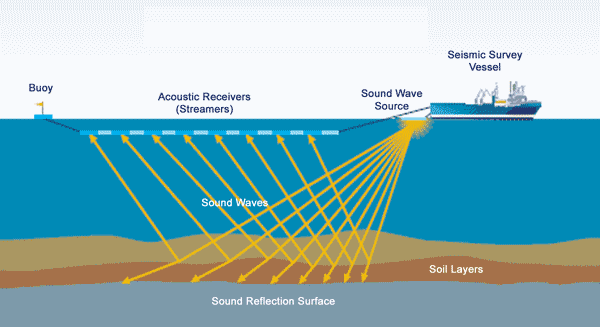
\includegraphics[width=0.8\textwidth]{fig/seismic_survey}
  \caption{Método de sísmica de reflexão \citep{figsismica}}
  \label{fig:1sismica}
\end{center}
\end{figure}


Para inversão acústica, o modelo mais utilizado para representar a resposta do
pulso sísmico atravessando as interfaces entre rochas é o convolucional. Nele é
assumido um modelo em camadas para a subsuperfície e ângulo de incidência e
reflexão de $90^\circ$. A medida efetuada é representada pelo resultado da
convolução do pulso sísmico, também chamado de \textit{wavelet}, com as
refletividades das interfaces. Os coeficientes de reflexão com ângulo de
reflexão normal são modelados por \citep[p. 69]{sen_livro}:

\begin{equation}
r(t) = \frac{z(t+\delta t)-z(t)}{z(t+\delta t)+z(t)}
\end{equation}
onde $z(t)$ é a impedância acústica no tempo $t$ definida por
$z(t)=\rho(t)v(t)$, onde $\rho(t)$ é a densidade da rocha e $v(t)$ a
velocidade de propagação da onda acústica. Utilizando os coeficientes de
reflexão, modela-se a resposta do sistema $d(t)$ aplicando a convolução
da \textit{wavelet} $s$ com os coeficientes de refletividade:

\begin{equation}
d(t) = \int_{-\infty}^{\infty} s(\tau)r(t-\tau)d\tau + e_d(t)
\end{equation}
onde é assumida a presença de um ruído aleatório $e_d(t)$ e $d$ é o chamado dado
sísmico. Cada sequência de dados $d$ representa um ponto no plano $xy$ e suas
posições $(t)$ são coordenadas em tempo que se relacionam com a profundidade.
Cada $d_{xy}$ é muitas vezes chamado de traço sísmico, o que no caso discreto
pode ser uma coluna de uma matriz 2D, por exemplo. Um conjunto de traços
sísmicos também é chamado de uma imagem, seção ou cubo, no caso de um
levantamento 3D. A \textit{wavelet} ideal seria um pulso tipo delta contendo
todas as frequências, mas gerar tal pulso não é viável. Na prática as
\textit{wavelets} são pulsos de banda limitada entre $6Hz$ e $65Hz$, o que
limita a frequência da sísmica e sua resolução \citep[p. 11]{sen_livro}.
A Figura \ref{fig:wavelet} ilustra uma \textit{wavelet} típica extraída de dados
reais.

\begin{figure}[htp]
\begin{center}
  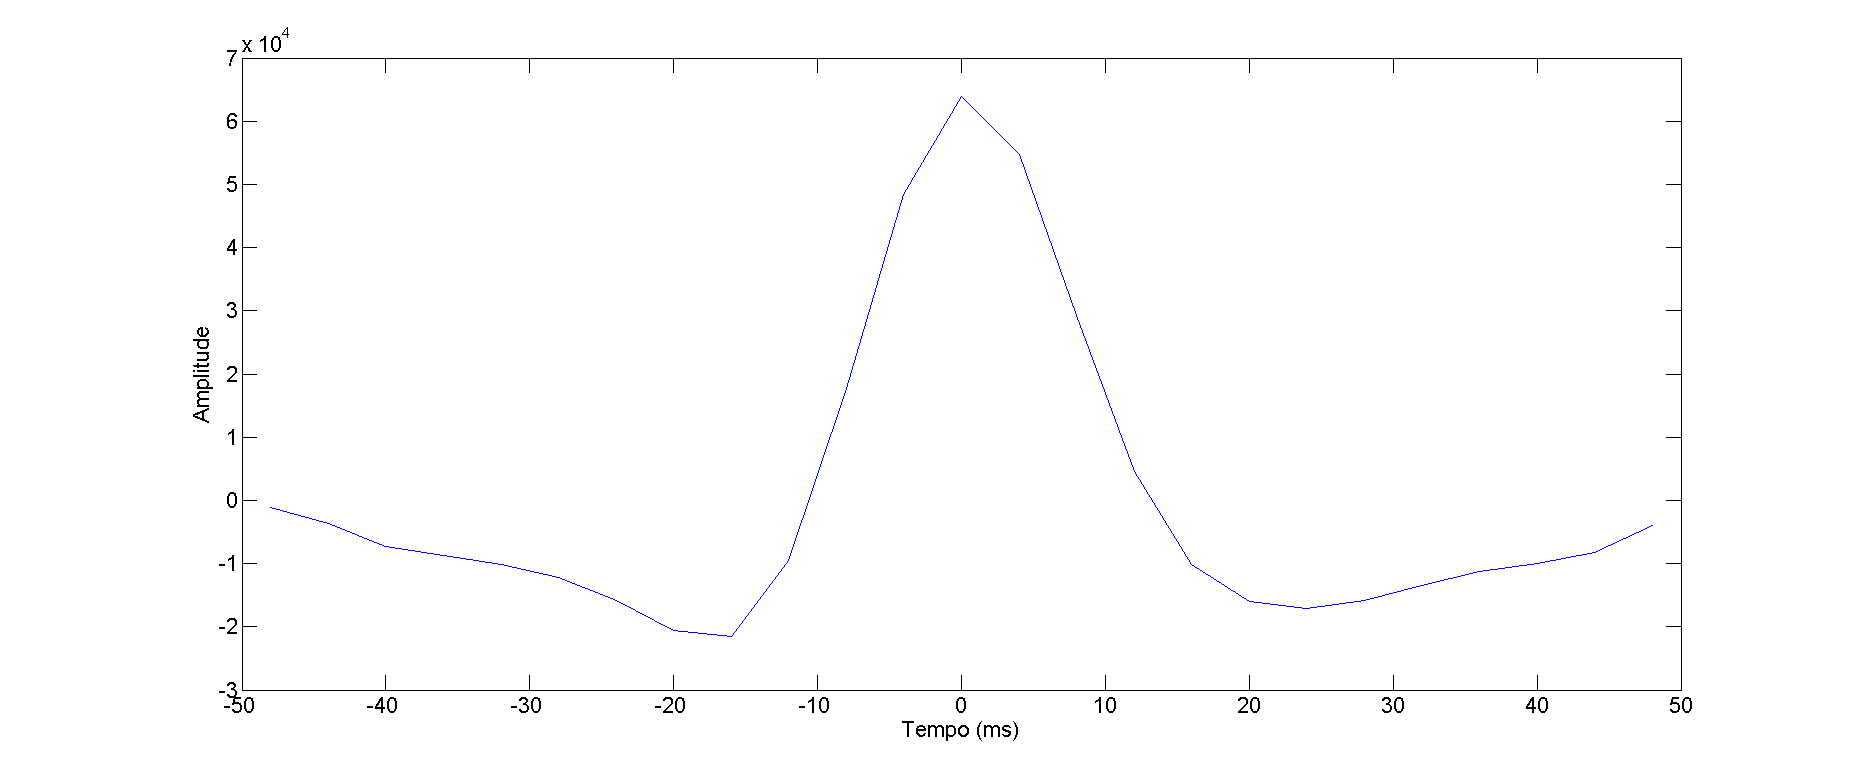
\includegraphics[width=0.8\textwidth]{fig/wavelet}
  \caption{\textit{Wavelet} extraída de dados reais}
  \label{fig:wavelet}
\end{center}
\end{figure}

O objetivo da inversão sísmica acústica é determinar os valores de impedância
acústica das camadas de rocha. Esse é um problema não linear, pois as equações
que determinam o modelo direto são não lineares. Também é considerado mal posto,
pois é ambíguo, ou seja, várias combinações de camadas e suas impedâncias podem
gerar o mesmo resultado no dado sísmico. Essas características geram a
necessidade de alta intervenção de especialistas para restringir o resultado
(regularização). Quando poços são perfurados, são utilizadas outras ferramentas
para observar dados mais próximos aos reais. Os principais métodos de inversão
utilizam os dados de poços para regularização e geração de estatísticas.

No processo de inversão é importante a modelagem da incerteza dos resultados
obtidos, ou seja, obter soluções equivalentes respeitando os dados medidos e as
informações \textit{a priori}. Essas soluções devem representar bem a região
onde o erro é menor que a tolerância desejada, chamada de região de equivalência
\citep{tompkins_comparisonBayes}. Existem várias razões para essa região de
equivalência existir, incluindo erros nas medidas, cobertura dos dados sobre a
as localizações desejadas, limitação de banda do pulso sísmico, suposições sobre
o modelo físico (e.g. isotropia, modelo de camadas, homogeneidade, etc.) e
aproximações matemáticas do modelo direto. A modelagem de incerteza ajuda na
avaliação dos riscos envolvidos nos processos de perfuração, exploração e
produção de óleo e gás.

As médias e variâncias locais das soluções não são suficientes para caracterizar
a incerteza na inversão, pois os modelos de impedância geralmente são utilizados
como entrada de processos como a simulação de fluxo. Esse tipo de simulação é
essencialmente uma função não linear, ou seja, a média das simulações de fluxo
não é necessariamente igual a simulação da média das impedâncias:
$F(\overline{\mathbf{m}})\neq \overline{F(\mathbf{m})}$, onde ${\mathbf{m}}$
representa as soluções aceitáveis, $F(\cdot)$ a função não linear da
simulação de fluxo e $ \overline{(\cdot)}$ a operação de média. Amostragem, de
uma forma geral, possibilita análises mais sofisticadas da distribuição
posterior \citep{hansenGibbsPrior}.

%TODO importancia das realizações na modelagem, ainda falta citação da
% simulacao de fluxo (funcao nao linear)

 Na literatura recente, diversos métodos foram propostos para tentar solucionar
 o problema da inversão sísmica com modelagem de incerteza.
Modelos envolvendo técnicas de inteligência computacional foram propostos para
tentar resolver o problema
\citep{senSimulatedAnnealin,MallickGeneticInve,max_inv_simulated,Artun2011143,MartinezPSO,Sambridge22102013}.
Apesar de terem oferecido bons resultados, esses modelos baseados em otimização
não capturam de forma ideal o conhecimento do especialista. A incerteza
resultante desses métodos é relacionada com o nível em que foi explorada a
superfície de erro, ao invés da incerteza relacionada aos dados e conhecimentos
\textit{a priori} inseridos.

O uso de ferramental probabilístico baseado no teorema de Bayes pode ser
aplicado, em conjunto com o amostrador de Gibbs, para gerar realizações
estocásticas da distribuição \textit{a posteriori} \citep{leandro_SEG}. Assim,
pode-se computar estatísticas do conjunto de soluções, obtido à alto custo
computacional. Para atacar a maldição da dimensionalidade e diminuir o custo da
amostragem de soluções, foram propostos métodos que utilizam redução dimensional
\citep{TompkinsScalabUnce2011}. Neste caso, aplicando análise de componentes
principais (PCA) é possível reduzir a dimensão do problema e utilizar um esquema
de amostragem determinística, ao custo de perda na resolução espacial das
amostras.

\section{Simulação Multiponto}



\section{Redes Neurais Convolucionais}
Nesta seção a convolução será descrita. Serão apresentados os principais conceitos relacionados às redes
neurais convolucionais e sua estrutura e as principais
aplicações deste modelo de aprendizagem de máquina. Um ponto não abordado nesta seção é
como escolher a arquitetura de uma rede convolucional.

As redes convolucionais, também chamadas de redes neurais convolucionais (CNN),
são um tipo de rede neural especializada em processamento de dados que possuam uma
topologia conhecida e em forma de grade. Exemplos deste tipo de dado são as séries
temporais, que podem ser vistas como uma grade em uma dimensão (1D) com amostras
em intervalos de tempo regulares, e dados de imagem, que podem ser pensados como
uma grade 2D de \textit{pixels}. As redes convolucionais são um tipo de rede neural
que usa a operação de convolução no lugar de multiplicação de matrizes em pelo menos uma
de suas camadas.

\subsection{Convolução}

A operação de convolução costuma ser denotada com um asterisco (Eq. \ref{eq:1}).
Na Equação. \ref{eq:1}, $x$ refere-se ao conjunto de imagens de entrada, uma sequência multidimensional
de dados, e $w$ é denominado \textit{kerenl} ou filtros, uma sequência multidimensional de parâmetros otimizados pelo algoritmo
de aprendizagem.
\begin{equation}
 s(t) = (x * w)(t)
 \label{eq:1}
\end{equation}

A convolução se sustenta sobre três pilares: interações esparsas, compartilhamentos
de parâmetros e representações equivalentes. As redes neurais tradicionais
utilizam a multiplicação de matriz por uma matriz de parâmetros para descrever
a interação entre cada unidade de entrada e cada unidade de saída. Isso
significa que toda unidade de saída interage com toda unidade de entrada.
As redes convolucionais, por outro lado, tipicamente possui interações
esparsas, também chamadas d conectividade esparsa ou pesos esparsos.
Para isto, é necessários que os filtros sejam menores que a entrada.
De um ponto de vista prático, no processamento de uma imagem,
a imagem de entrada pode ter milhares de pixels, entretanto, é 
possível detectar apenas pequenas regiões de características importantes,
por exemplo com significado geológico, com filtros que compreendam apenas
algumas dezenas ou centenas de pixels na imagem. Como consequência,
menos parâmetros são armazenados e aumenta a eficiência estatística do
modelo. As figuras \ref{fig:full} e \ref{fig:sparse} ilustram
os modelos citados anteriormente. É possível notar que o número de elementos
que afetam elemento de saída em destaque ($s_3$) é definido pela convolução
com filtro de largura 3 (figura \ref{fig:sparse}), por outro lado $s_3$ é
afetado por todos os elementos da entrada quando formado por multiplicação
matricial (figura \ref{fig:full}).

\begin{figure}[htp]
\begin{subfigure}{.5\textwidth}
  \centering
  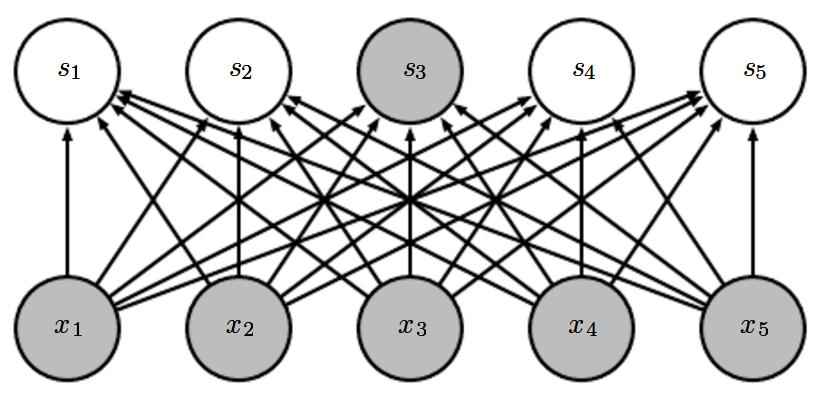
\includegraphics[width=.9\linewidth]{fig/full_conections}
  \caption{Conectividade tradicional.}
  \label{fig:full}
\end{subfigure}%
\begin{subfigure}{.5\textwidth}
  \centering
  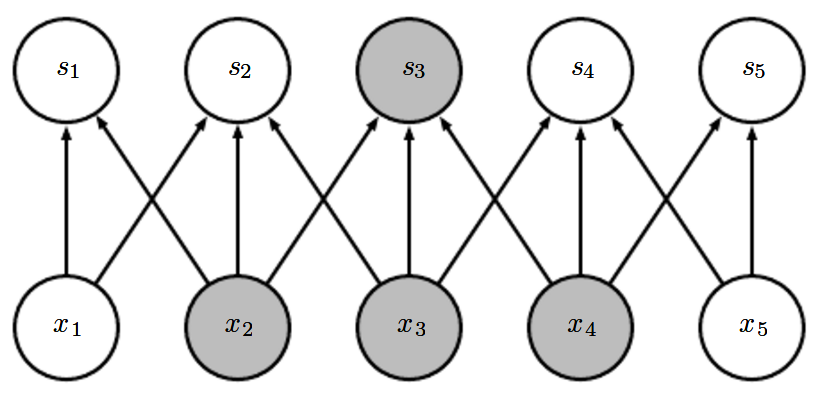
\includegraphics[width=.9\linewidth]{fig/sparse_conections}
  \caption{Conectividade esparsa.}
  \label{fig:sparse}
\end{subfigure}
\end{figure}

O \textbf{compartilhamento de parâmetros}, também chamado de \textbf{pesos amarrados} 
em uma rede convolucional se refere ao uso do mesmo parâmetro para mais de uma função no modelo.
Nas redes neurais tradicionais, cada elemento da matriz de pesos é usado apenas uma vez quando a
saída da camada é calculada, pois é multiplicado por apenas um elemento da entrada. No compartilhamento
de pesos, o valor do peso aplicado a uma entrada está relacionado ao valor de um peso aplicado em
algum outro local. Na rede convolucional, cada elemento do filtro é usado em toda posição da entrada,
de modo que, ao invés de aprender um conjunto separado de parâmetros toda localização da imagem, apenas
um conjunto é aprendido.

\subsection{Pooling}
Uma camada em uma rede convolucional consiste de três estágios. No primeiro estágio,
a camada realiza diversas convoluções para produzir um conjunto de ativações lineares.
O segundo estágio é chamado etapa de detecção, na qual cada ativação é submetida a uma
função não-linear. A terceira etapa é chamada de \textit{pooling}, responsável por
modificar a saída para o resumo estatístico das saídas em uma determinada vizinhança. A operação de
\textit{pooling} permite tornar invariante pequenas translações no conjunto de entrada,
ou seja, ainda que haja pequenas translações na entrada, os valores da maioria das saídas após a
o \textit{pooling} permanecem iguais. A figura \ref{fig:pool} ilustra o funcionamento da função de \textit{pooling}.
\begin{figure}[htp]
\begin{center}
  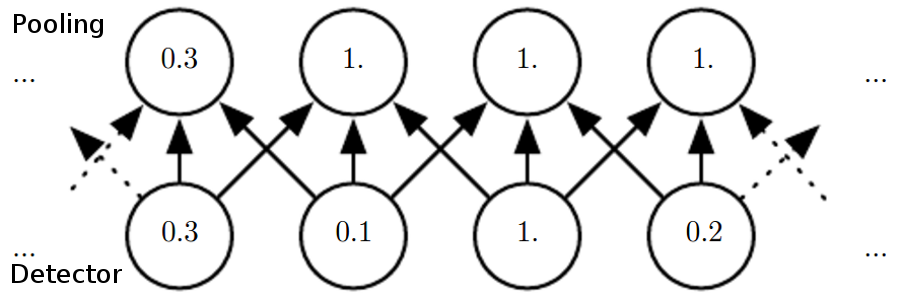
\includegraphics[width=0.7\textwidth]{fig/pool}
  \caption{Operação de \textit{pooling} com região de tamanho 3. Nesta operação é selecionado o máximo valor de ativação da etapa de detecção.}
  \label{fig:pool}
\end{center}
\end{figure}

A operação de \textit{pooling} permite lidar com entradas de tamanho variável.
Classificar imagens de tamanhos diferentes, por exemplo, pode ser realizado
variando o tamanho entre as regiões de pooling de modo que a camada de 
de classificação sempre receba o mesmo número de sumários estatísticos
independente do tamanho da imagem.

\section{Objetivo}

O objetivo do presente trabalho consiste em propor um modelo capaz de integrar a
atualização Bayesiana no processo de inversão GSI. Resultados prévios indicam
que utilizar ...

Outro objetivo é ...

\section{Organização do Texto}

Este documento está organizado da seguinte forma. Após esta breve introdução, o
Capítulo \ref{cap:2modelosInversao} apresenta o estado da arte em modelos de
inversão sísmica com modelagem de incerteza. O Capítulo \ref{cap:3modeloHibrido}
trata da proposta do projeto e resultados preliminares da integração de
atualização Bayesiana em inversão Geoestatística, a ser desenvolvido em parceria
com o CERENA - Centro de Recursos Naturais e Ambiente do Instituto Técnico da
Universidade de Lisboa, sob orientação do professor Dr. Amilcar Soares,
especialista em Geoestatística e inversão sísmica. O estágio será iniciado em
julho de 2015 e terá 12 meses de duração. Após o retorno ao Brasil, estão
planejados mais 8 meses de trabalho para finalizar a escrita da tese e defesa.



%Modelos para Inversão Sísmica com Modelagem de Incerteza
\chapter{Fundamentação Teórica}
\label{cap:2fundamentacao}
Neste capítulo o problema inverso será apresentado
em linhas gerais e a inversão sísmica será abordada em maiores detalhes.
Serão apresentados os conceitos relacionados a \textit{Deep Learning}, assim como os
elementos de redes neurais convolucionais. Esta fundamentação
teórica é relevante para o entendimento de como o modelo de rede neural convolucional
pode ser adotado para obter ganho qualitativo e quantitativo no pós-processamento
da inversão sísmica.

\section{Problema Inverso}
A teoria de inversão é utilizada em diversas áreas para inferir os valores de
parâmetros relacionados com processos físicos a partir de um conjunto de dados medidos,
os quais são chamados dados experimentais. É possível descrever o problema inverso
como o processo de obter informações de um sistema parametrizado, a partir de
dados que podem ser medidos por meio de algum experimento físico e das relações teóricas com os parâmetros
desejados, mas que não são passíveis de medição. Frequentemente, algum conhecimento \textit{a priori}
é incorporado ao modelo.

Um sistema físico depende do domínio em estudo. Pode ser uma galáxia para um
astro-físico, pode ser a Terra para um geofísico ou uma partícula quântica
para um físico quântico. Em comum, o fato de que, para ser estudado, um sistema
físico segue três passos básicos: a parametrização do sistema, a modelagem direta e a modelagem inversa \citep{tarantola}.
A parametrização do sistema se refere à definição do conjunto mínimo de elementos (parâmetros)
cujos valores caracterizam completamente o sistema. A escolha dos parâmetros do modelo geralmente
é não única, de modo que dois conjuntos de parâmetros diferentes podem ser equivalentes.

A modelagem direta significa prever os valores dos parâmetros observáveis (dados $d$),
que correspondem a um dado modelo (conjunto de parâmetros $m$). Esta predição pode ser denotada
pela Eq. \ref{eq:frdmdl}. Onde $F(.)$ é chamado operador direto.
\begin{equation}
\label{eq:frdmdl}
d = F(m) 
\end{equation}

Por sua vez, a modelagem inversa se refere ao uso de resultados atuais das medições dos parâmetros
físicos observáveis, para inferir os valores atuais dos parâmetros do modelo (não-observáveis).
O problema inverso pode ser descrito em uma forma discreta como:
\begin{equation}
\label{eq:deqgm}
m = F^{-1}(d)
\end{equation}
onde, $F$ é o sistema físico investigado, e relaciona os parâmetros do modelo $m=(m_1, m_2,...,m_n) \subset R^n$
estimado com os dados observados $d \in R^s$.
Como mencionado no Capítulo \ref{cap:1intro}, um problema inverso possui múltiplas soluções,
de modo que o modelo $m$ pertence a um conjunto de modelos $M$ admissíveis.
Na prática, $d$ pode ser uma função no domínio do tempo e/ou espaço, ou pode ser
uma coleção de observações discretas.

\section{Inversão Sísmica}
Os métodos geofísicos frequentemente envolvem a solução e avaliação de problemas inversos,
pois permitem inferir a distribuição das propriedades físicas na subsuperfície da Terra
usando observações a partir da superfície. A inversão sísmica tem um papel fundamental na solução 
de problemas geofísicos, em especial na caracterização de reservatórios \citep{Bosch2010,Srivastava2009}.
Do ponto de vista prático, as soluções para o problema de inversão sísmica melhoram a exploração e
o gerenciamento na indústria petrolífera, uma vez que os dados sísmicos estimados possuem forte correlação com as
propriedades petrofísicas (porosidade, densidade, etc.) das rochas da subsuperfície \citep{Figueiredo2014}.
Para facilitar o entendimento da inversão sísmica, considere a subsuperfície como sendo formada por camadas
sobrepostas de diferentes tipos de rochas. As regiões onde ocorrem as transições entre tipos
diferentes de rochas são chamadas de \textit{facies} e possuem espessuras diferentes.

\subsection{Aquisição Sísmica}
O dado sísmico é o principal parâmetro observável utilizado na inversão sísmica.
A aquisição destes dados se dá por meio da sísmica de reflexão. Este
método utiliza pulsos sísmicos de uma fonte artificial controlada e monitora a resposta em
função do tempo. Neste sistema, cada região de contato entre dois tipos de rochas
diferentes gera reflexão e refração do pulso sísmico, como demonstrado na Figura
\ref{fig:1sismica}.
De um ponto de vista bastante elementar, é possível intuir que a parte refletida da onda se
propaga em todas as direções, de modo que os componentes horizontal e vertical podem ser medidos.
O componente horizontal (\textit{s-wave}), referente à reflexão horizontal
da onda, é utilizado no processo de inversão conhecido como inversão elástica. Por outro lado, o componente
vertical da onda (\textit{p-wave}), referente à reflexão vertical do pulso emitido, é utilizado no processo
conhecido como inversão acústica.
\begin{figure}[ht!]
\begin{center}
  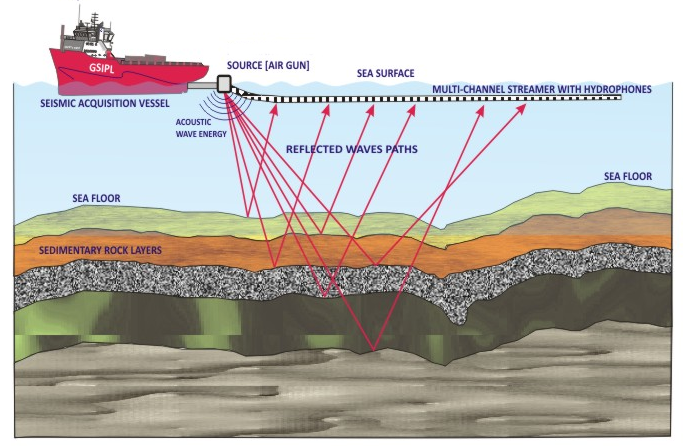
\includegraphics[width=0.8\textwidth]{fig/seismic_survey_2}
  \caption{Método de sísmica de reflexão \citep{figsismica}}
  \label{fig:1sismica}
\end{center}
\end{figure}

O pulso de onda emitido durante a aquisição possui um formato próprio, uma identidade, 
conhecido como \textit{wavelet}. Assim, a resposta sísmica medida
é composta em parte por esta identidade e, em parte, pela característica da interface
entre duas camadas de rochas diferentes, na qual o pulso reflete.
Esta característica é chamada de coeficiente de refletividade (Equação \ref{eq:refletv}):
\begin{equation}
r(t) = \frac{z(t+\delta t)-z(t)}{z(t+\delta t)+z(t)}
\label{eq:refletv}
\end{equation}
onde, $z(t)$ é a impedância acústica no tempo $t$ definida por
$z(t)=\rho(t)v(t)$, onde $\rho(t)$ é a densidade da rocha e $v(t)$ a
velocidade de propagação da onda acústica.
O dado sísmico utilizado na inversão acústica, portanto,
é uma aproximação da resposta da camada terrestre. Pode ainda ser definido como
a convolução entre a \textit{wavelet} de aquisição e o valor de refletividade entre as
camadas, com ângulo de incidência e reflexão de $90^\circ$,
respectivamente. Por este motivo, este modelo é chamado convolucional.
Com os coeficientes de reflexão e a discretização da medida de tempo, é possível
modelar o dado sísmico $d(t)$ aplicando a convolução $*$
da \textit{wavelet} $s$ com os coeficientes de refletividade $r$:
\begin{equation}
d(t) = s(\tau) * \sum_{j-1}^{N}{r(t- t_j) \delta(t - t_j) + e_d(t)}
\end{equation}
onde $N$ é o número total de camadas, $e_d(t)$ representa o ruído aleatório em função do tempo
e cada $d_{xy}$ é chamado de traço sísmico. Um conjunto de traços
sísmicos também é chamado de imagem, seção ou cubo, no caso de um
levantamento 3-D. A \textit{wavelet} ideal seria um pulso tipo delta contendo
todas as frequências, entretanto, na prática as
\textit{wavelets} são pulsos de banda limitada entre $6Hz$ e $65Hz$, o que
limita a frequência da sísmica e sua resolução \citep[p. 11]{sen_livro}.
Como consequência, as imagens resultantes do processo de inversão também terão
o seu espectro de frequência limitado. A Figura \ref{fig:wavelet} ilustra uma
\textit{wavelet} típica extraída de dados reais.
\begin{figure}[htp]
\begin{center}
  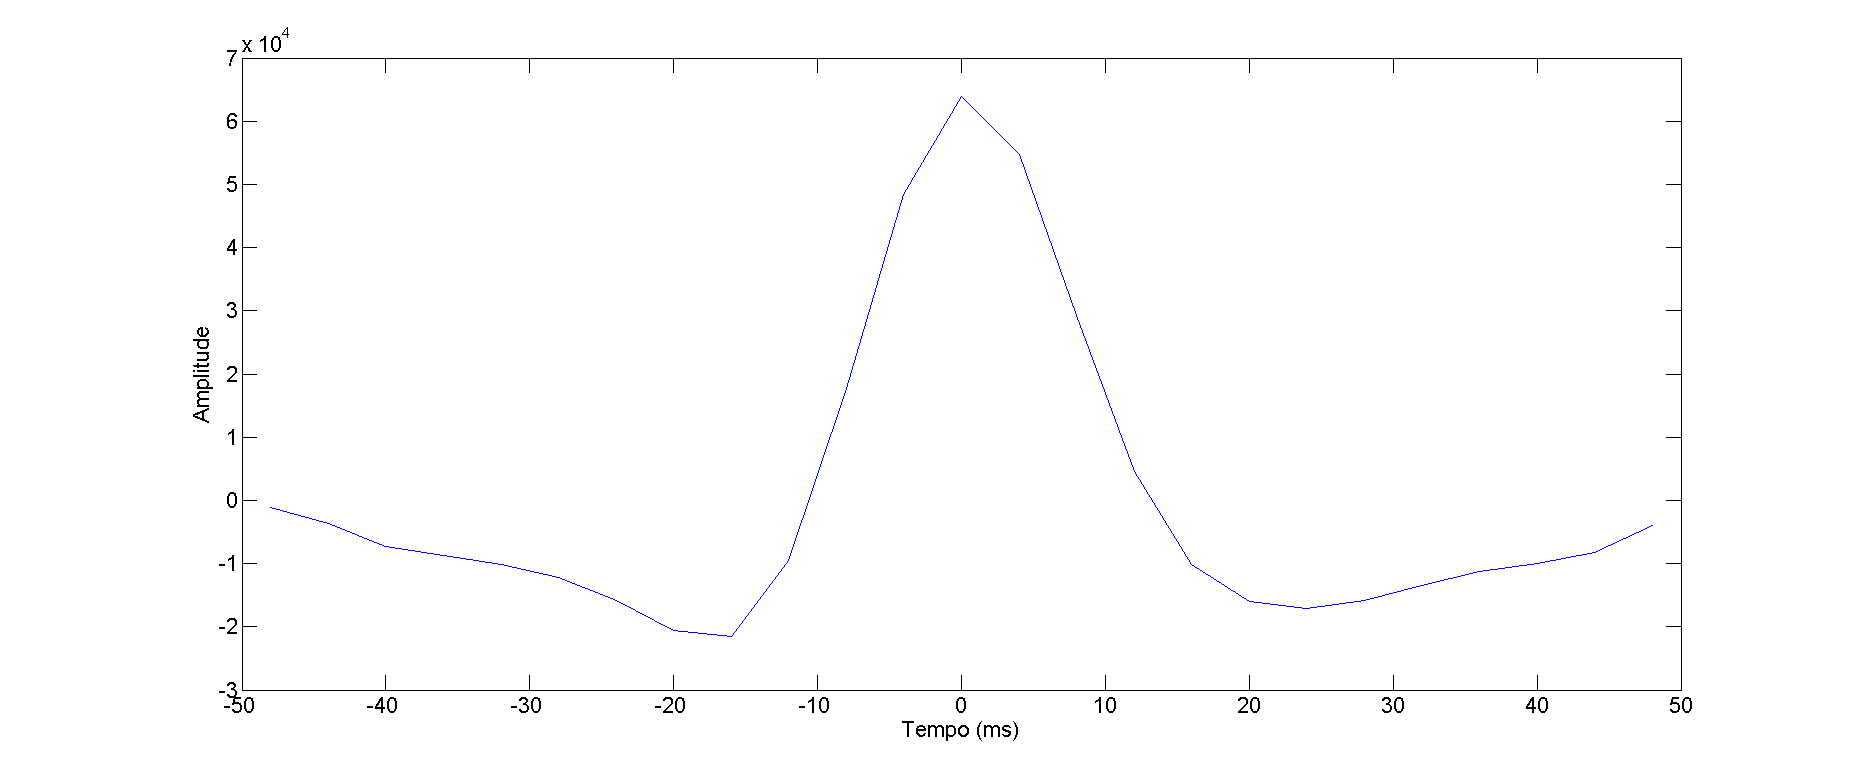
\includegraphics[width=0.8\textwidth]{fig/wavelet}
  \caption{\textit{Wavelet} extraída de dados reais}
  \label{fig:wavelet}
\end{center}
\end{figure}

\section{Redes Neurais Convolucionais}
As Redes Neurais Convolucionais (RNC), também chamadas de redes convolucionais,
são um tipo de rede neural especializada em processamento de dados que possuem uma
topologia conhecida e em forma de grade \citep{Gdfl16}. Exemplos deste tipo de dado são as séries
temporais, que podem ser vistas como uma grade em uma dimensão (1-D) com amostras
em intervalos regulares de tempo, e dados de imagem, que podem ser vistos como
uma grade (2-D) de \textit{pixels}. Este modelo de rede neural é chamado convolucional,
pois emprega a operação de convolução no lugar de multiplicação comum entre matrizes,
em pelo menos uma de suas camadas.

\subsection{Convolução}
A operação de convolução é definida como a integral do produto de duas funções após uma delas sofrer um
certo deslocamento. Considere o exemplo em que se deseja rastrear a localização de uma
nave espacial com um sensor a laser. O sensor disponibiliza uma saída $x(t)$ referente à posição da nave
no tempo $t$. Ambos, $x$ e $t$, são valores reais, de modo que uma saída diferente pode ser obtida
em qualquer instante de tempo. Considerando que o sensor possui um certo ruído, para realizar uma
estimativa mais precisa da posição da nave é preciso ponderar várias medidas de posição juntas.
Como os valores medidos mais recentemente são mais relevantes, se estima uma função peso
$w(a)$, onde $a$ é o tempo de medição. Se esta média ponderada for aplicada a todos os instantes,
a estimativa de posição da nave será suavizada:

\begin{equation}
 s(t) = \int{x(a) w(t-a)da}.
 \label{eq:1}
\end{equation}

A convolução costuma ser denotada com um asterisco e aplicada com o tempo $t$ discretizado para valores inteiros,
dada da seguinte forma:
\begin{equation}
 s(t) = (x * w)(t) = \sum_{a=-\infty}^{\infty}{x(a)w(t-a)}.
 \label{eq:2}
\end{equation}
No contexto das redes convolucionais, $x$ se refere ao conjunto de imagens de entrada 
e $w$ é denominado \textit{kernel} ou filtros. As imagens de entrada são uma sequência multidimensional 
de dados, enquanto os filtros são uma sequência multidimensional de parâmetros a serem 
otimizados pelo algoritmo de aprendizagem.
Nos casos em que o problema compreende imagens $X$ e filtros $W$ utilizados em duas dimensões 
a convolução ganha o seguinte formato:
\begin{equation}
 S(i,j) = (X*W)(i,j) = \sum_{m}\sum_{n}{X(m,n)W(i-m,j-n)}.
\end{equation}

Nas redes convolucionais há pelo menos duas estruturas básicas, a camada convolucional e a camada de \textit{pooling}.
A arquitetura típica de uma RNC compreende duas camadas convolucionais, cada uma seguida por
uma camada \textit{pooling}, como ilustrado na Figura \ref{fig:cnn_basic_arq}. À medida que as imagens progridem
ao longo da rede, suas dimensões diminuem, entretanto, elas se tornam mais profundas
em termos de hierarquia de conceitos extraídos. No topo da pilha de camadas da rede
se adiciona camadas completamente conectadas, sendo que na última camada ocorre a saída prevista.
Esta estrutura de camadas completamente conectadas é a mesma utilizada nas redes neurais tradicionais
do tipo \textit{feedforward}, nas quais todos os nerônios de uma camada estão conectados a todos os
neurônios da camada seguinte. 
\begin{figure}[htp]
\begin{center}
  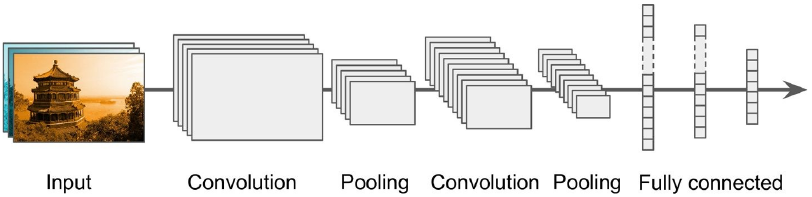
\includegraphics[width=0.8\textwidth]{fig/cnn_basic_arq}
  \caption{Arquitetura típica de uma rede neural convolucional. \citep{aurelien17}}
  \label{fig:cnn_basic_arq}
\end{center}
\end{figure}

A camada convolucional é o elemento mais importante de uma RNC. Esta camada é estruturada
de modo a fazer com que cada um dos seus neurônios esteja conectado a um 
pequeno grupo de \textit{pixels} da camada de entrada (Figura \ref{fig:cnn_arq}) e não a todos os \textit{pixels}, como
ocorre em redes neurais tradicionais. Cada neurônio da camada seguinte se conecta apenas aos neurônios
contidos em uma pequena região da camada anterior e assim sucessivamente. Esta região que define
o grupo de neurônios conectados ao neurônio da próxima camada é chamada \textbf{campo perceptivo}.
Este formato permite o aprendizado de características de baixo nível na primeira camada e de
características de mais alto nível nas camadas seguintes.
\begin{figure}[htp]
\begin{center}
  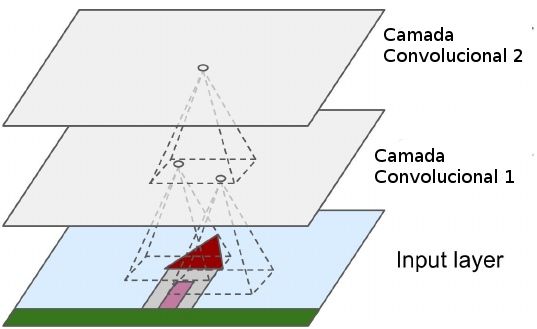
\includegraphics[width=0.6\textwidth]{fig/cnn_arq}
  \caption{Camadas de uma RNC com campos receptivos retangulares.}
  \label{fig:cnn_arq}
\end{center}
\end{figure}

A Figura \ref{fig:cnn_stride} ilustra  um exemplo de campo receptivo e das conexões entre duas camadas em uma rede convolucional.
Considere um neurônio localizado na linha $i$ e coluna $j$ de uma dada camada.
Este neurônio estará conectado às saídas dos neurônios da camada anterior
localizados nas linhas ${i}\times{s_h}$ até ${i}\times{s_h}+f_h - 1$, colunas
${j}\times{s_w}$ até ${j}\times{s_w}+f_w - 1$, onde
$f_h$ e $f_w$ são a altura e a largura do campo receptivo, $s_h$ e $s_w$
são os deslocamentos vertical e horizontal ao longo das imagens da camada anterior.
O tamanho destes deslocamentos é chamado de passo ou \textit{stride}
e quanto maior o \textit{stride}, menor será a imagem resultante na camada seguinte. Para \textit{stride}
de tamanho $0$ a camada seguinte terá as mesmas dimensões da camada anterior.
\begin{figure}[htp]
\begin{center}
  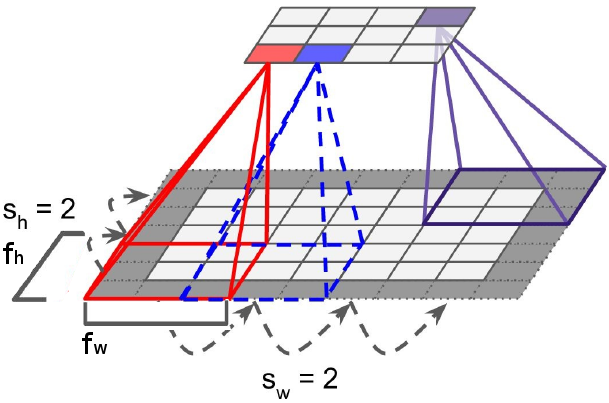
\includegraphics[width=0.6\textwidth]{fig/cnn_layer_stride_2}
  \caption{Conexão entre camadas com campo receptivo 3 x 3 e \textit{strides} de tamanho 2.}
  \label{fig:cnn_stride}
\end{center}
\end{figure}

\subsection{Filtros}
Os filtros (pesos) em uma camada convolucional são representados como uma pequena
imagem com as mesmas dimensões do campo receptivo. São eles os elementos
convolvidos com a imagem de entrada para obter o resultado da camada convolucional.
Durante o treinamento de uma rede convolucional cada elemento dos filtros é otimzado.
A Figura \ref{fig:conv_filt} ilustra dois filtros exemplos e o resolutado da convolução
de cada um com uma certa imagem. O primeiro filtro é um quadrado preto
(\textit{pixels} de valor 0) contendo uma coluna central branca (\textit{pixels} com valor 1). 
Analogamente, o segundo filtro é um quadrado preto contendo uma linha central branca.
É possível notar na imagem da esquerda que as linhas verticais brancas se tornaram mais
evidentes, enquanto as outras partes da imagem se tornaram mais borradas. Na imagem da direita 
a convolução com o filtro horizontal destacou as linhas brancas horizontais, ao passo que
o restante ficou borrado. Assim, quando uma característica é detectada por um neurônio, ela representa
o tipo de padrão da entrada que causará a sua ativação.
Estes padrões podem ser bordas, contornos ou estruturas com outras formas.
\begin{figure}[htp]
\begin{center}
  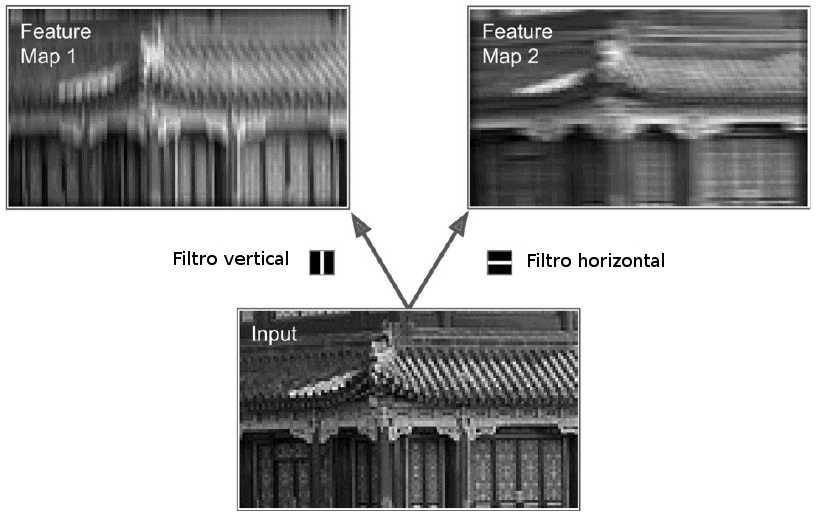
\includegraphics[width=0.7\textwidth]{fig/conv_filt}
  \caption{Aplicação de dois filtros diferentes para obter mapas de características.}
  \label{fig:conv_filt}
\end{center}
\end{figure}

Em situações reais, a camada convolucional possui muitos mapas de características, resultando
em uma representação em 3-D como ilustrado na Figura \ref{fig:featmaps}. Os mapas de características
de uma camada convolucional são o resultado da convolução de uma das imagens de entrada com os diversos
filtros específicos desta camada, de modo que, é possível imaginar que à medida que o número de imagens aumenta,
a estrutura ilustrada se replica horizontalmente.
\begin{figure}[htp]
\begin{center}
  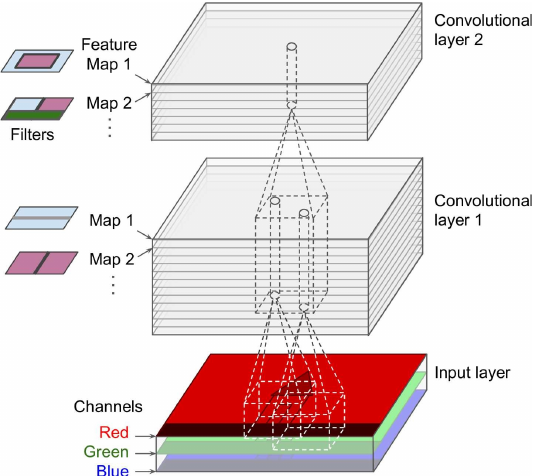
\includegraphics[width=0.6\textwidth]{fig/feat_maps}
  \caption{Camadas convolucionais com múltiplos mapas de características e imagens com três canais.}
  \label{fig:featmaps}
\end{center}
\end{figure}

\subsection{Pooling}
O processamento ao longo de uma rede convolucional ocorre em três estágios. No primeiro estágio
acontecem as convoluções entre as imagens e os filtros, para produzir um conjunto de ativações lineares.
O segundo estágio é chamado estágio de detecção, na qual cada ativação é submetida a uma
função não-linear. O terceiro estágio é chamado de \textit{pooling}, responsável por
modificar a saída da camada convolucional para obter um sumário estatístico das saídas da convolução.
Semelhante ao que ocorre na convolução, a região sobre a qual se aplica o \textit{pooling} é definida por um
campo receptivo e o deslocamento é definido por um \textit{stride}. O \textit{pooling} permite tornar
invariante pequenas translações no conjunto de entrada, ou seja, ainda que haja pequenas translações na
entrada, os valores da maioria das saídas após o \textit{pooling} permanecem iguais.
A Figura \ref{fig:pool} ilustra o funcionamento da função de \textit{pooling} máximo, na qual
o máximo valor de ativação dentro de uma vizinhança é selecionado. Outras funções de \textit{pooling} incluem o valor médio
dentro de uma região retangular, a normalização $L2$ de uma vizinhança, ou a média ponderada baseada na distância do \textit{pixel} central.
\begin{figure}[htp]
\begin{center}
  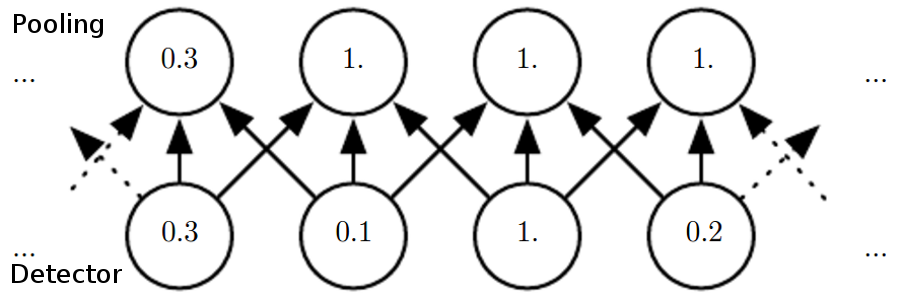
\includegraphics[width=0.7\textwidth]{fig/pool}
  \caption{Operação de \textit{pooling} com campo receptivo de tamanho $3$. Nesta operação é selecionado o máximo valor de ativação da etapa de detecção.}
  \label{fig:pool}
\end{center}
\end{figure}

A propriedade de invariância é útil quando a existência de uma característica é mais relevante que
o local exato onde ela ocorre. Por exemplo, para determinar se o rosto de uma pessoa ocorre em uma certa imagem, não é necessário saber
com precisão o local dos olhos, basta saber se há um olho do lado esquerdo do rosto e outro olho do lado direito
\footnote{O rosto da figura pública Nestor Cerveró, por exemplo, seria facilmente identificável por uma rede convolucional com uma camada de \textit{pooling}}.
Por outro lado, há contextos em que o local da característica é uma informação relevante e deve ser preservada. 
Por exemplo, em modelagem de reservatórios, a detecção de bordas referentes a uma facie selante sobre uma região de reservatório.
Adicionalmente, a operação de \textit{pooling} permite lidar com entradas de tamanho variável. Na classificação de imagens,
as entradas para a camada classificadora devem ter o mesmo tamanho. Assim, o \textit{stride} entre regiões de \textit{pooling} pode variar
para que a camada classificadora receba o mesmo número de sumários estatísticos, independente do tamanho das imagens.

As função de \textit{pooling} sumariza as respostas de vizinhanças separadas por $k$ \textit{pixels}, por isso, o tamanho do seu campo receptivo é menor
que o campo receptivo da convolução. Isto aumenta a eficiência computacional da rede, pois a camada seguinte à de \textit{pooling} terá $k$ vezes
menos entradas para processar. Quando o número de filtros da camada seguinte é função do tamanho da sua entrada, a redução promovida pela
função de \textit{pooling} pode resultar em maior eficiência estatística e redução da quantidade de memória \citep{aurelien17}.

\subsection{Propriedades das Redes Convolucionais}
Por conta da sua arquitetura, as redes convolucionais se sustentam sobre três pilares: interações esparsas, compartilhamentos
de parâmetros e representações equivariantes. As propriedades de interação esparsa e compartilhamento de pesos serão apresentados
em maiores detalhes nesta seção, embora já tenham sido introduzidos de forma intuitiva nas seções anteriores.

As \textbf{interações esparsas}, também chamadas de conectividade esparsa ou pesos esparsos,
ocorre quando os filtros possuem dimensão menor que a entrada, ou seja, a
dimensão do campo receptivo é menor que a dimensão das imagens de entrada.
De um ponto de vista prático, a imagem de entrada pode ter milhares de \textit{pixels}, entretanto, é 
possível detectar apenas pequenas regiões com características de maior relevância na imagem de entrada
com filtros que compreendam apenas algumas dezenas \textit{pixels}.
Por exemplo, é possível identificar características de uma face humana no reconhecimento de pessoas, ou estruturas com
significado geológico em um estudo geofísico. As Figuras \ref{fig:sparse} e \ref{fig:full} ilustram
os modelos de conectividade esparsa e não-esparsa, respectivamente.
É possível notar que na conectividade não-esparsa (Figura \ref{fig:full}) todos os elementos da camada inferior
afetam o elemento em destaque $s_3$ da camada seguinte, enquanto na conectividade esparsa (Figura \ref{fig:sparse}) apenas
três elementos afetam o elemento em destaque. O número de elementos que afetam o elemento em destaque na
conectividade esparsa é definido pelo tamanho do filtro utilizado na convolução.
\begin{figure}[htp]
\begin{subfigure}{.5\textwidth}
  \centering
  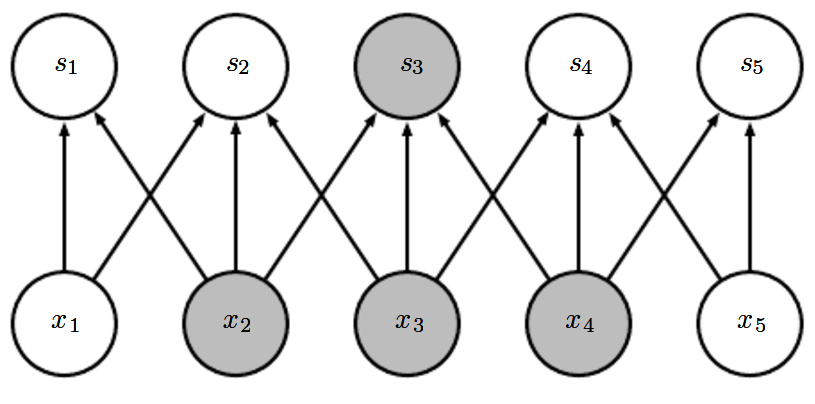
\includegraphics[width=.9\linewidth]{fig/sparse}
  \caption{Conectividade esparsa.}
  \label{fig:sparse}
\end{subfigure}
\begin{subfigure}{.5\textwidth}
  \centering
  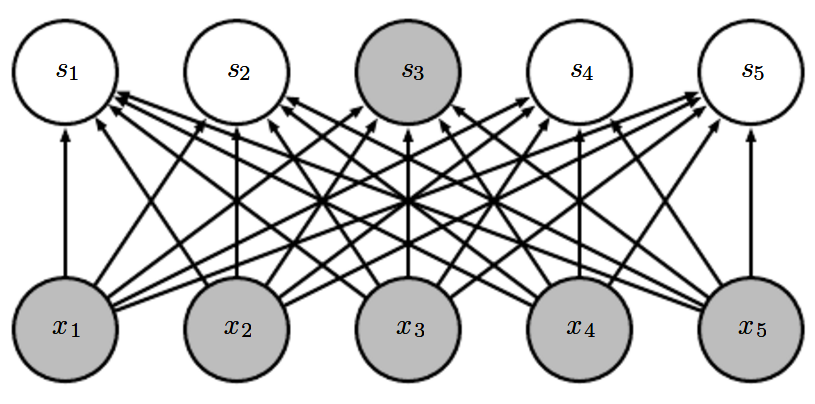
\includegraphics[width=.9\linewidth]{fig/full}
  \caption{Conectividade tradicional.}
  \label{fig:full}
\end{subfigure}%
\end{figure}

O \textbf{compartilhamento de parâmetros}, também chamado de \textbf{pesos amarrados},
se refere ao uso do mesmo parâmetro para mais de uma função no modelo.
Como já mencionado, nas redes neurais tradicionais todos os neurônios de uma camada são conectados a todos os neurônios
da camada anterior e cada neurônio possui um \textit{bias}, como ilustrado na imagem \ref{fig:shallow}.
Entretanto, este modelo é pouco eficiente, pois não tira vantagem da estruturas espaciais das imagens
de entrada \citep{Gdfl16}.
\begin{figure}[htp]
\begin{center}
  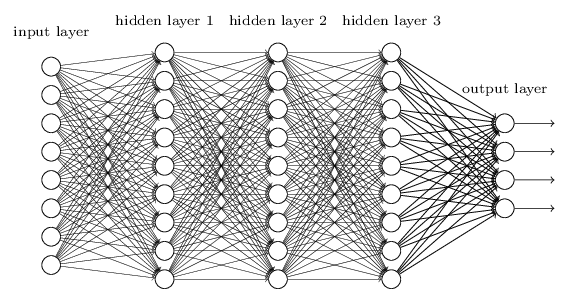
\includegraphics[width=0.7\textwidth]{fig/shallow_nn}
  \caption{Organização de camadas de uma rede neural do tipo \textit{feedforward}.}
  \label{fig:shallow}
\end{center}
\end{figure}
Parece senso comum que estas informações estruturais são muito relevantes em problemas geoestatísticos, afinal as imagens
neste domínio representam estruturas geológicas.

No compartilhamento de pesos a saída de cada neurônio
de uma camada depende apenas do conjunto de neurônios de uma pequena região definida pelo campo receptivo da camada anterior:
\begin{equation}
 {\sigma} \times \bigg( b + \sum_{m}\sum_{n}{w_{m,n}a_{i+m,j+n} \bigg) }
\end{equation}
onde, $\sigma$ é uma função de ativação, $b$ é o valor compartilhado do \textit{bias}, $w_{m,n}$ é
uma matriz de pesos compartilhados (filtros) e $a_{i+m,j+n}$ denota a entrada $a_{x,y}$ na posição
$x,y$. Como o mesmo filtro é convolucionado ao logo da imagem,
os mesmos pesos e \textit{bias} aprendem diferentes características da imagem. Deste modo, cada conjunto de pesos e \textit{bias} é compartilhado
por diferentes regiões em cada imagem e o número de pesos conectados ao neurônio
da camada seguinte diminui em relação ao modelo tradicional. Isto faz com que a convolução seja mais eficiente que a multiplicação de matriz
do ponto de vista de requisitos de memória e eficiência estatística.

O compartilhamento de pesos confere às redes convolucionais a propriedade de \textbf{equivariância} de
translação. Se uma função é equivariante, significa que se a entrada muda,
a saída muda igualmente. Matematicamente, a função $f(x)$ é equivariante à função $g$ se
$f(g(x)) = g(f(x))$. No caso da convolução, se $g$ é uma função que translada a entrada, então
a convolução será equivariante a $g$.
A convolução com imagens cria um mapa 2-D dos locais onde certas características aparecem na entrada.
A propriedade de equivariância permite rastrear objetos transladados na entrada. Se um objeto aparece
em uma determinada posição e, em seguida, aparece em outra posição, sua representação
irá mover a mesma quantidade na saída. É importante frisar que, nas RNC, a propriedade de equivariância
é aplicável apenas para a translação, de modo que a convolução não é equivariante para transformações 
de escala e rotações na imagem.

\section{Resumo}

Este Capítulo detalhou os principais conceitos abordados neste trabalho. O
problema inverso foi introduzido e a inversão sísmica apresentada em
maiores detalhes. Foram apresentados os elementos que compõem as redes
neurais convolucionais: a convolução, as camadas convolucionais, os filtros e a camada de \textit{pooling}.
Foram apresentadas também as propriedades das camadas convolucionais: conectividade esparsa,
compartilhamento de parâmetros e equivariância de translação. O Capítulo seguinte apresenta a
revisão do estado da arte para inversão sísmica e para os modelos de RNC utilizados para Super-resolução.

%Integração de 
\chapter{Revisão da Literatura}
\label{cap:3revisaoliteraria}

Neste capítulo serão apresentadas as revisões relacionadas
ao método de inversão acústica e aos modelos de super-resolução de imagens.
Esta revisão evidenciou o potencial de pesquisa desta proposta, pois
apresenta uma lacuna em métodos de pós-processamento da inversão sísmica.
Para esta revisão sistemática foram consultados os portais \textit{Google Scholar}, \textit{Science Direct} e \textit{IEEE Xplore}.
As buscas tiveram o alcance de dez anos e foram usadas as seguintes palavras-chaves: \textit{Deep Learning},
\textit{Convolutional Neural Network}, \textit{Super-resolution}, \textit{Seismic Inversion},
\textit{Acoustic Inversion}. Com estas palavras-chaves foram definidas as seguintes \textit{queries} para consulta nos periódicos:

\begin{itemize}
 \item ((Convolutional neural networks OR deep learning OR super-resolution) AND (seismic inversion OR acoustic inversion)).
 \item ((Convolutional neural networks OR deep learning) AND (super-resolution AND seismic inversion)).
 \item ((deep learning OR Convolutional neural networks) AND (seismic inversion)).
 \item ((super-resolution AND seismic inversion))
\end{itemize}

Embora não estejam diretamente relacionados com super-resolução pós-inversão sísmica,
os textos encontrados com as \textit{queries} listadas ajudaram a agregar novas ideias
a este trabalho e contribuíram para o desenvolvimento desta proposta. 
\cite{ZhaoSAE29} apresentam um estudo comparativo sobre os métodos supervisionados e
não-supervisionados para classificação de fáceis. Os autores abordam os métodos
de PCA, Mapas Auto-organizáveis, Mapas Topográficos, Redes Neurais Artificiais do tipo \textit{feed-forward} e 
Máquina de Vetor de Suporte. Neste trabalho os autores sugerem o uso de métodos não-supervisionados
em detrimento dos supervisionados, para evitar problemas de representação da variação litológica e estratigráfica
devido à insuficiência de dados para o treinamento do modelo.

O trabalho proposto por \cite{Korjani16} apresenta uma abordagem, baseada em rede neural,
na qual utiliza os dados de um conjunto de poços vizinhos para prever
propriedades sintéticas de um poço hipotético em uma região qualquer do campo em estudo.
Embora a abordagem adotada utilize um conjunto massivo de dados com $425$ poços de treinamento
e $48$ poços para teste, o modelo de rede neural propriamente dito não apresenta características de \textit{Deep Learning}.
O método sugere o uso dos poços com menor distância até o local onde se deseja simular os dados. Os dados dos poços
selecionados são usados em um modelo de rede do tipo \textit{Feed-forward} multi-camadas.

A observação da literatura mostra que o uso de RNC é uma abordagem recente na solução de problemas inversos.
Dentre os trabalhos encontrados com a revisão sistemática, é possível destacar
o uso de RNC na reconstrução interativa de imagens de tomografia computadorizada para lidar
com a degradação de imagens em aquisições curtas e com o desconforto do paciente em aquisições longas \citep{Hwan16}. 
Os autores questionam os aspectos teóricos e práticos na comparação entre os métodos tradicionais de
reconstrução de imagens e o método por RNC, e ressaltam que RNC pode ser um bom ajuste para lidar com
problemas inversos inerentemente convolucionais.

Mais recentemente, um modelo de RNC foi desenvolvido para realizar classificação de fáceis a partir de dados
sísmicos pré-empilhados. O modelo apresentado por \cite{Qian17} é uma rede auto-codificadora (\textit{autoenconder})
capaz de aprender características de dados sísmicos pré-empilhados e supera a Análise de Componentes Principais (ACP)
na remoção de redundâncias e extração de informações válidas. As características extraídas pela RNC são submetidas a um algoritmo
de classificação para obter o reconhecimento de fácies. O problema de inversão de litofácies com dados pré-empilhados também foi
abordado por \cite{Lihui2017} por meio da combinação de dois métodos de \textit{Deep Learning}: \textit{Deep Belief Network} (DBN)
e \textit{Restricted Boltzmann} (RBM).
O modelo proposto superou as limitações relacionadas ao uso de redes neurais tradicionais na inversão de litofácies. Os autores
descrevem estas limitações como convergência local, resultados instáveis e inaplicabilidade das redes neurais tradicionais para 
conjuntos de dados extensos. O modelo não-supervisionado RBM foi treinado com as litofácies conhecidas e com dados de atributos
sísmicos de todas as camadas, desta forma o modelo definiu relacionamentos entre atributos sísmicos e fácies classificadas.
Em seguida, um modelo DBM de aprendizado de litofácies foi definido de modo que as litofácies foram
calculadas em toda a extensão do dado sísmico, com isto o modelo reduziu a incerteza na inversão de camadas finas
em diferentes bandas de frequência da sísmica.

De acordo com \cite{Xiaoyu2012}, um caminho
para melhorar a resolução da inversão sísmica é adicionar alta frequência
na aquisição e processamento do dado sísmico. Entretanto, expandir a reflexão de alta frequência é uma tarefa
difícil por conta de fatores como atenuação da terra, ruído de alta frequência, 
entre outros. Ainda segundo o estudo, o dado sísmico com baixa frequência e
sem parte da alta frequência ($0 - 0 - 60 - 120Hz$) gera erro na parte da mutação da impedância, o que
influencia na resolução e precisão do resultado da inversão sísmica. O dado sísmico
sem a baixa frequência e sem parte da alta frequência ($10 - 20 - 60 - 120Hz$) causa erro na parte de transição da impedância
contínua, mas não na parte de mutação da impedância. Isto sugere que a ausência da baixa frequência influencia
na tendência vertical do resultado da inversão \citep{Xiaoyu2012}. Por outro lado, a inversão na qual o dado sísmico possui baixas e
altas frequências ($0 - 0 - 100 - 300Hz$) é similar ao modelo geológico.
Assim, a estratégia sugerida neste trabalho objetiva a inserção de faixas de alta frequência no pós-processamento da propriedade invertida.
A hipótese deste trabalho é de que estas altas frequências podem ser obtidas em padrões existentes nas imagens de treinamento
e em seus respectivos dados sísmicos e que estes padrões podem ser aprendidos por um modelo de rede convolucional
para serem utilizados na reconstrução de imagens que não possuem altas frequências. Ainda, as altas frequências podem ser obtidas
a partir de dados de poços e a super-resolução pode ser realizada unidimensionalmente, um traço por vez.
Os modelos que representam o estado da arte em inversão acústica e redes convolucionais para super-resolução são discutidos nas seções a seguir.

\section{Métodos de Inversão Sísmica}
É importante ter em mente que, durante a inversão, as operações são realizadas
sobre dois espaços de representações diferentes: o espaço do modelo e o espaço de dados.
No contexto da inversão sísmica, os dados sísmicos são representados no espaço
dos dados. Para uma abordagem quantitativa, uma parametrização precisa ser definida \citep{tarantola} e,
no contexto da inversão acústica, o parâmetro do modelo adotado é a impedância acústica.
Para obter informações sobre os parâmetros do modelo, é necessário
realizar observações através de experimentos físicos, como por exemplo, a
aquisição sísmica.

É possível questionar por que não definir a
função inversa da modelagem direta e calcular, de forma imediata,
os parâmetros do modelo a partir do espaço dos dados.
No entanto, os métodos de inversão direta sofrem de instabilidades
devido ao ruído e características do problema \citep[p. 50]{sen_livro}. Outra
opção é utilizar tentativa e erro para ajustar os parâmetros até conseguir uma
resposta semelhante aos dados experimentais. Formalmente isto é automatizado
utilizando métodos de otimização. Para tanto é preciso definir uma função
objetivo, que meça o ajuste dos dados produzidos pelos
parâmetros do modelo (dado sintético) ao dado medido.

\subsection{Inversão Sísmica Linear e Não Linear}
O conteúdo desta seção apresenta as suposições de linearidade necessárias
que tornam a inversão acústica um processo analítico e computacionalmente
eficiente. O detalhamento matemático pode ser consultado em \cite{leandroGRSL,Figueiredo17}.

É importante ter em mente
que os problemas inversos podem ser classificados de acordo com a natureza
do relacionamento entre os dados e o modelo, e de acordo com o comportamento da função objetivo \citep{sen_livro}.
Assim, eles podem ser: linear, fracamente não-linear, quasi-linear e não-linear.
Na maioria dos problemas geofísicos o operador direto $G$ é não-linear.
Assim como nos algoritmos de aprendizagem de máquina, na inversão sísmica
a não-linearidade implica em uma função de custo com forma complicada,
possivelmente com mínimos locais.
Por outro lado, se o operador $G$ for aproximadamente linear, a
função de erro se tornará quadrática em relação a perturbações
no espaço do modelo. A maior parte da teoria de inversão é baseada em problemas
de inversão linear e, em muitas aplicações, ela é 
adequada para representar a natureza do sistema \cite{sen_livro}.

O modelo sísmico direto pode ser representado pelo modelo convolucional dado por:
\begin{equation}
d(t) = \int_{-\infty}^{\infty} s(\tau) r(t - \tau)\mathrm{d}\tau + e_{d}(t),
\label{eq:conmodel}
\end{equation}
onde $d(t)$ é o traço sísmico, $s(t)$ é a \textit{wavelet}, $e(t)$ é
um ruído aleatório e $r(t)$ é a refletividade.
A representação discreta para o modelo convolucional do dado sísmico é
dada pela operação matricial: 
\begin{equation}
\label{eq:sismDiscreta}
\mathbf{d = Sr + e},
\end{equation}
onde $\mathbf{S}$ é uma matriz convolucional construída utilizando uma
\textit{wavelet}, $\mathbf{r}$ é a matriz de refletividades e $e$ é um
ruído admitido. Em teoria, o ruído é uma interferência aleatória que não se tem
controle, na prática se considera ruído tudo que não é explicado pela função
$G$, e.g. imprecisões no modelo físico e problemas com filtragem e processamento
dos dados.

Para escapar da problemática da não-linearidade do operador direto, é
necessário aproximar linearmente o pulso sísmico da impedância acústica.
Para isto, duas medidas são necessárias. A primeira é admitir a 
refletividade como o logaritmo da impedância acústica (Equação \ref{eq:lnz}).
Esta aproximação é válida para valores de refletividade menores que $0.3$.
\begin{equation}
r(t) = \frac{1}{2}\Delta \ln(z(t)).
\label{eq:lnz}
\end{equation}
A segunda medida, é adotar um operador diferencial $\textbf{D}$. Assim,
se define o operador linear $\textbf{G=(1/2)SD}$ e o modelo $m=ln(z)$.
Com isto, a relação entre o dado sísmico e o parâmetro do modelo (impedância acústica)
se torna linear por:
\begin{equation}
\label{eq:sismDiscreta2}
\mathbf{d = Gm + e}.
\end{equation}

Quando não é possível o uso da aproximação da Equação \ref{eq:lnz}, o problema
deve ser abordado utilizando métodos de otimização não-linear. Com isso os erros
devido às aproximações do modelo \textit{forward} diminuem, mas a otimização se
torna mais custosa. Como a relação entre os dados e os parâmetros é não linear, a
função objetivo a ser minimizada terá mínimos locais, tornando necessário
o uso de métodos de otimização global. Esta prática está bem documentada na
literatura de inversão, como o uso de \textit{simulated annealing}
\citep{max_inv_simulated}, de algoritmos genéticos \citep{MallickGeneticInve} e
enxame de partículas \citep{zhe_nonlinear}. 

\subsection{Máximo \textit{a posteriori}}
\label{sec:map}

A teoria mais simples e genérica possível é obtida quando se usa uma
abordagem probabilística \citep{tarantola}. Na solução para a inversão
sísmica, os parâmetros do modelo convolucional da equação \ref{eq:sismDiscreta2}
podem ser representados em termos de suas distribuições de probabilidade.
No modelo estocástico proposto por \cite{leandroGRSL}, as distribuições
são consideradas normais e multivariadas e são denotadas por $N(\boldsymbol{\mu},\boldsymbol{\Sigma})$.
Assumindo que o ruído $\boldsymbol{e}$ respeita uma distribuição também gaussiana,
as distribuições de probabilidade para o vetor dos dados sísmicos experimentais
$\boldsymbol{d}$, para a \textit{wavelet} $\boldsymbol{w}$ e para
o vetor dos parâmetros do modelo $\boldsymbol{m}$ são
definidos, respectivamente, pelas distribuições \ref{eq:psismico}, \ref{eq:pwavelet} e \ref{eq:pmodelo}.

\begin{equation}
\label{eq:psismico}
p(\boldsymbol{d}|\boldsymbol{\mu_{d}},\boldsymbol{\Sigma_{d}}) =
N(\boldsymbol{\mu_{d}},\boldsymbol{\Sigma_{d}}),
\end{equation}
onde $\boldsymbol{\mu_{d}} = \boldsymbol{Gm}$ é o vetor com a sísmica
sintética e $\boldsymbol{\Sigma_{d}}$ é a matriz de covariância do ruído da
sísmica, a qual é definida conforme a confiabilidade que o especialista tem no
dado sísmico ou seu nível de ruído.

\begin{equation}
\label{eq:pwavelet}
p(\boldsymbol{s}|\boldsymbol{\mu_{s}},\boldsymbol{\Sigma_{s}}) =
N(\boldsymbol{\mu_{s}},\boldsymbol{\Sigma_{s}}),
\end{equation} 
onde o valor esperado da \textit{wavelet} $\boldsymbol{\mu_{s}}$ é definido
como um vetor nulo. Para que o método possa ser aplicado para a inversão
acústica, é necessário estimar uma \textit{wavelet} que possa ser aplicada
no modelo convolucional. Esta estimativa é realizada aplicando este mesmo processo
de inversão na região de ocorrência de amostragem de dados, um poço perfurado por exemplo, onde a refletividade pode
ser calculada diretamente \citep{leandroGRSL}. O algoritmo de
Gibbs então é utilizado para amostrar na distribuição posterior da \textit{wavelet}, 
o valor médio e a variância são calculados.

\begin{equation}
\label{eq:pmodelo}
p(\boldsymbol{m}|\boldsymbol{\mu_{m}},\boldsymbol{\Sigma_{m}}) =
N(\boldsymbol{\mu_{m}},\boldsymbol{\Sigma_{m}}).
\end{equation} 
Na representação da distribuição dos parâmetros do modelo é possível inserir no método de inversão, informações \textit{a priori}
que eventualmente estejam disponíveis. Por exemplo, $\boldsymbol{\mu_{m}}$ pode ser
uma matriz de baixa frequência gerada a partir da interpolação da impedância acústica observada em dois poços
já perfurados \citep{leandroGRSL}.

A inversão por Máximo \textit{a posteriori} (MAP)
\citep{Buland01012003,leandroGRSL} é realizada para cada traço individualmente.
As distribuições condicionais e o modelo convolucional apresentados anteriormente
são as estruturas necessárias para realizar a inversão acústica. O ponto de partida
é a aplicação do próprio método para estimar a \textit{wavelet},
com ela é possível estimar as distribuições de probabilidades envolvidas no modelo.
Em seguida, basta calcular a exponencial do modelo convolucional para obter a distribuição posterior
para o parâmetro do modelo, que no caso em questão é a impedância acústica. Esta distribuição é dada por:

\begin{equation}
p(\boldsymbol{m}|\boldsymbol{d_{o}},\boldsymbol{s},\boldsymbol{\mu_{m}},\sigma_{d}^{2},\sigma_{m}^{2}) = 
N(\boldsymbol{\mu_{m|}},\boldsymbol{\Sigma_{m|}}).
\end{equation} 

A média e variância posterior para cada traço podem ser calculadas analiticamente via \citep{leandroGRSL}:

\begin{equation}
\label{eqn:mapSolution}
\boldsymbol{\mu}_{m|} = \boldsymbol{\mu}_{m} + \boldsymbol{\Sigma}_{m}\boldsymbol{G}^{T}(\boldsymbol{G\Sigma}_{m}\boldsymbol{G}^{T}+\boldsymbol{\Sigma}_{d})^{-1}\left ( \boldsymbol{d}_{o} - \boldsymbol{G\mu}_{m} \right ),
\end{equation}
\begin{equation}
\boldsymbol{\Sigma}_{m|} = \boldsymbol{\Sigma}_{m} - \boldsymbol{\Sigma}_{m}\boldsymbol{G}^{T}(\boldsymbol{G\Sigma}_{m}\boldsymbol{G}^{T}+\boldsymbol{\Sigma}_{d})^{-1}\boldsymbol{G\Sigma}_{m},
\end{equation} 
onde o cálculo da matriz inversa acima pode ser aproveitado para vários traços
de uma região de interesse, em certos casos, ou seja, quando as matrizes de
covariância podem ser assumidas iguais para todos os traços da sísmica da região.
Desta forma se alteram a sísmica $\mathbf{d}_0$ e a baixa frequência
$\boldsymbol{\mu_m}$ e se obtém a média posterior para o traço desejado.
  
A matriz de covariância posterior indica a incerteza
presente no resultado. Não é necessário
definir a tolerância de ajuste aos dados, mas é preciso definir a
matriz de covariância do resultado esperado, ou seja, é
preciso ter conhecimento, mesmo que de forma grosseira, das correlações espaciais e
variâncias que se espera do resultado. Outro ponto relevante é o fato da
solução para o método de inversão MAP ser expressa em termos da covariância
e do valor esperado. Com isto as imagens de impedância acústica obtidas
se caracterizam por serem suavizadas, principalmente na região de
transição entre camadas. Durante a convolução, a \textit{wavelet} funciona
como uma modeladora, de modo que as altas frequências são filtradas
e o nível de detalhes das imagens se torna limitado. 

\section{Métodos de Super-resolução de Imagens}
Super-resolução é o processo para gerar uma ou mais imagens de alta
resolução a partir de uma ou mais imagens de baixa-resolução
através do aumento no número de \textit{pixel} por unidade de área \cite{Nasrollahi2014}.
Os algoritmos de super-resolução têm aplicação nas mais diferentes áreas
tais como, processamento de imagens aéreas e de satélite, reconhecimento de
íris, holografia digital, melhoramento de imagens faciais e de texto, entre
outras. Os modelos de super-resolução podem ser classificados
de acordo com diferentes fatores como: o domínio de aplicação,
o número de imagens de baixa resolução aplicadas e o método de reconstrução \citep{Nasrollahi2014}.

Métodos baseados em interpolação são fáceis de implementar e amplamente utilizados,
entretanto estes métodos sofrem de falta de expressividade, uma vez que modelos lineares
não são capazes de expressar dependências complexas entre as entradas e as saídas \citep{HsiehAndrews1978}.
Na prática, tais métodos falham na tentativa de prever adequadamente detalhes de alta frequência,
levando a saídas de alta resolução borradas. Efeito semelhante ocorre durante a inversão sísmica,
na qual as imagens resultantes apresentam resolução limitada e contornos borrados.

\subsection{Super-resolução por RNC}

Os algoritmos de super-resolução realizam buscas por
fragmentos de estruturas e os combinam para criar detalhes
de alta frequência \citep{Freeman2002,Huang2015}. Há abordagem no sentido
de melhorar os métodos de interpolação simples através da construção
de dicionários de filtros pré-treinados e selecionar os fragmentos
por algum algoritmo de \textit{Hashing} \citep{Romano2017}. O algoritmo citado
representa o estado da arte dos métodos baseados em interpolação, cujo foco está na
velocidade de inferência. As redes convolucionais, por outro lado,
focam na construção das imagens de alta resolução, de modo a obter magnitudes
cada vez maiores de detalhes.

As redes convolucionais extraem implicitamente
múltiplas camadas de abstração através da otimização dos seus filtros.
Elas são capazes de modelar a distribuição conjunta sobre
uma imagem $x$ como o produto de distribuições condicionais \citep{Oord16}:
\begin{equation}
\label{eqn:prodcnn}
p(x) = \prod_{i=1}^{n^2}p(x_i|x_1,...,x_{i-1})
\end{equation}
onde, $x_i$ é o pixel modelado. A imagem é percorrida linha por linha e cada
\textit{pixel} depende apenas dos \textit{pixels} localizados em uma vizinhança pré-determinada.
Para garantir esta propriedade se define uma máscara para os filtros da convolução,
ou seja, é atribuído valor $0$ para os pesos fora da zona de interesse.
A nova imagem é gerada sequencialmente, cada \textit{pixel} é reinserido para a rede para que o próximo seja previsto,
deste modo cada \textit{pixel} depende dos \textit{pixels} anteriores
sob uma perspectiva não-linear.

O modelo condicional sofreu melhorias que permitiram o reconhecimento de estruturas mais complexas.
Entre as camadas convolucionais do modelo condicionado foram adicionadas unidades
multiplicativas com a seguinte ativação:
\begin{equation}
\label{eqn:actvcnn}
y = tanh(W_{k,f} * x)\odot \sigma(W_{k,g}*x)
\end{equation}
onde $\sigma$ é a função sigmoide, $k$ é o número da camada, $*$ é o operador
convolucional e $\odot$ é o produto membro a membro das duas matrizes. Este modelo é
conhecido como \textit{Gated PixelNN} \citep{Oord16}.

A Figura \ref{fig:example2} apresenta exemplos da aplicação do modelo condicional \textit{Gated PixelNN}
para realizar super-resolução.
A rede foi testada com duas configurações diferentes, contendo $10$ e $100$ gargalos na sua estrutura.
Na Figura \ref{fig:example2}, a coluna mais à esquerda apresenta a imagem real, a segunda coluna apresenta
o resultado para a rede auto-codificadora treinada com o Erro Quadrático Médio (MSE) e as
colunas seguintes apresentam as amostras obtidas pelo modelo \textit{Gated PixelNN}.
\begin{figure}[ht!]
\begin{center}
  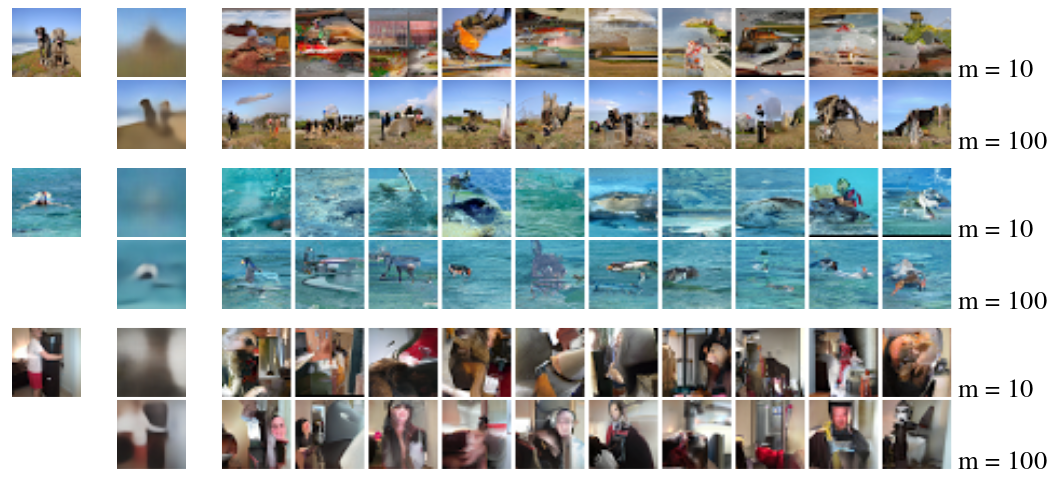
\includegraphics[width=0.8\textwidth]{fig/example_superres_2}
  \caption{Exemplo de aplicação do modelo probabilístico PixelNN. \citep{Oord16}}
  \label{fig:example2}
\end{center}
\end{figure}

O modelo de super-resolução é condicionado a um conjunto de
descrições $\boldsymbol{h}$, de modo que a distribuição condicional é dada
por:
\begin{equation}
\label{eqn:prodcnncond}
p(x|\boldsymbol{h}) = \prod_{i=1}^{n^2}p(x_i|x_1,...,x_{i-1}|\boldsymbol{h}).
\end{equation}
Desta forma, as ativações das camadas convolucionais dependem de $\boldsymbol{h}$,
antes de passarem pela função de não-linearidade. Se $\boldsymbol{h}$ contiver
informações referentes a classes de características encontradas nas imagens, todas as camadas terão um \textit{bias} que determina
a dependência destas classes. Por outro lado, se $\boldsymbol{h}$ for mapeado
para uma representação espacial $\boldsymbol{s}=m(\boldsymbol{h})$, onde $m$ é uma rede
deconvolucional, as camadas convolucionais terão \textit{biases} dependentes da localização
das estruturas contidas em $\boldsymbol{h}$, presentes na imagem. Assim, a equação \ref{eqn:actvcnn}
ganha a seguinte forma \citep{Oord16}:
\begin{equation}
\label{eqn:actvcnncond}
y = tanh(W_{k,f} * x + V_{k,f}*\boldsymbol{s})\bigodot \sigma(W_{k,g}*x + V_{k,g}*\boldsymbol{s}).
\end{equation}

O modelo de rede condicional proposto por \cite{DahlNS17} representa o estado da arte em modelos convolucionais para
super-resolução de múltiplas imagens. O modelo é composto de uma rede condicionante, do tipo ResNet \citep{He2016}
e uma rede \textit{prior}, do tipo \textit{Gated PixelNN} \citep{Oord16}.
A rede condicionante realiza o mapeamento de uma imagem de baixa resolução para uma estrutura probabilística
de alta resolução. Assim, ela permite compor a estrutura da imagem de alta resolução através da distribuição
de probabilidade marginal dos \textit{pixels} na imagem de baixa resolução. A rede \textit{prior} adiciona detalhes de alta resolução
para tornar as saídas mais realísticas. 

Para treinar um modelo que mapeie uma imagem $x$ de baixa resolução em uma imagem $y$ de alta resolução,
dada uma imagem $y^*$ considerada a realidade desejada, é preciso otimizar os parâmetros
$\theta$ da distribuição condicional $p_{\theta}(\boldsymbol{y}|\boldsymbol{x})$ de modo
a maximizar a função objetivo condicional dada por \citep{DahlNS17}:
\begin{equation}
\label{eqn:objfunc}
O(\theta|\mathcal{D})= \sum_{(\boldsymbol{x},\boldsymbol{y^*})\in \mathcal{D}} log p(\boldsymbol{y^*}|\boldsymbol{y}),
\end{equation}
onde $\mathcal{D} \equiv \{(\boldsymbol{x}^{(i)},\boldsymbol{y}^{*(i)})\}_{i=1}^N$ denota o conjunto
de treinamento da rede, composto pelos pares de imagens de baixa resolução e de alta resolução que representa
a realidade observada.

Dada uma imagem $ \boldsymbol{x} \in \mathbb{R}^L $, $A_i(\boldsymbol{x}) : \mathbb{R}^L \rightarrow \mathbb{R}^K$
representa a rede condicionante capaz de prever um vetor de valores que correspondem a $K$ valores
possíveis que o $i$-ésimo \textit{pixel} de saída pode assumir. Analogamente,
$B_i(\boldsymbol{y}_{<i}) : \mathbb{R}^{i-1} \rightarrow \mathbb{R}^K$ representa a rede \textit{prior}
capaz de prever um vetor de valores do $i$-ésimo \textit{pixel}. A previsão da distribuição
sobre o $i$-ésimo \textit{pixel} de saída é obtida pela adição dos dois conjuntos de saída e aplicação
do operador de \textit{softmax}:

\begin{equation}
\label{eqn:cnnpred}
p(y_i|\boldsymbol{x},\boldsymbol{y}_{<i}) = softmax(A_i(\boldsymbol{x}) + B_i(\boldsymbol{y}_{<i})).
\end{equation}
O operador \textit{softmax} é uma generalização da regressão logística. Na regressão logística se assume que a classificação 
admite um entre dois valores: $y^{(i)} \in \{ 0,1\}$. A regressão \textit{softmax} permite lidar com
$y^{(i)} \in \{ 0,...,K\}$, onde $K$  é o número de classes \citep{Nielson15}.

O algoritmo Gradiente Descente Estocástico é usado para otimizar os parâmetros $A$ e $B$, a fim de maximizar
a \textit{log-likelihood} da Equação \ref{eqn:objfunc}. O aprendizado da rede ocorre pela otimização da função de custo entre
as predições do modelo (Equação \ref{eqn:cnnpred}) e os valores discretos da imagem que representa
a realidade $y_i^* \in \{1...K\}$:

\begin{equation}
\label{eqn:cnncostfunc}
O = \sum_{(\boldsymbol{x},\boldsymbol{y^*})\in \mathcal{D}} \sum_{i=1}^{M}\big(\zeta [\boldsymbol{y_i^*}]^T(A_i(\boldsymbol{x}) + B_i(\boldsymbol{y}_{<i}^*))
-lse(A_i(\boldsymbol{x}) + B_i(\boldsymbol{y}_{<i}^*))) \big).
\end{equation}

Os experimentos realizados por \cite{DahlNS17} compreenderam o treinamento do modelo condicionado
com o conjunto de dados \textit{CelebA} \citep{liu15}, o qual é composto por $200K$ imagens de
faces de pessoas consideradas celebridades. Os autores redimensionaram as imagens de
$32$ x $32$ para $8$ x $8$ para obter a mesma imagem, porém borrada. Com isto, os
pares de treinamento da rede foram formados. A Figura \ref{fig:example1} apresenta um exemplo
de resultado obtido pelo modelo proposto. A coluna da esquerda mostra as imagens de baixa
resolução, em tamanho $8$x$8$, usadas como entrada para o modelo, a coluna central mostra o
resultado obtido com o modelo, em tamanho $32$ x $32$, e a coluna da direita apresenta o imagem
real.
\begin{figure}[ht!]
\begin{center}
  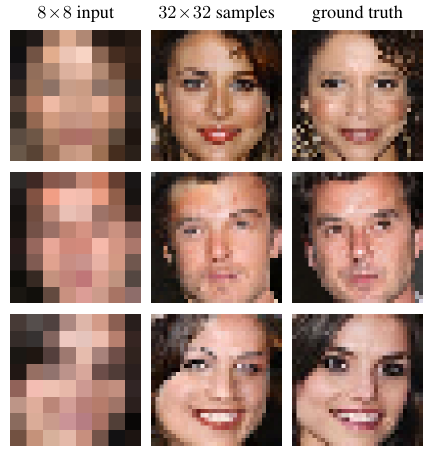
\includegraphics[width=0.4\textwidth]{fig/example_superres_1}
  \caption{Ilustração do modelo probabilístico. \citep{DahlNS17}}
  \label{fig:example1}
\end{center}
\end{figure}

Mais recentemente, os avanços das pesquisas do Google em \textit{Deep Learning} disponibilizaram
ferramentas de implementação de diferentes algoritmos de aprendizagem de máquina. Dentre estas
ferramentas está o \textit{Framework} de \textit{Deep Learning} TensorFlow, no qual os modelos
de redes convolucionais podem ser implementados e testados.

\section{Resumo}

Neste capítulo foram revisados os estados da arte em inversão sísmica acústica e modelos
de rede convolucional para super-resolução.
O próximo capítulo irá definir a proposta de pesquisa, apresentar os resultados preliminares, o plano de trabalho e concluir com as perspectivas de
contribuição.





%=============================== Bibliografia ===============================================
\addcontentsline{toc}{chapter}{Bibliografia}
\renewcommand{\bibname}{Bibliografia}
\markboth{Bibliografia}{Bibliografia}

\bibliographystyle{my-agsm}
\bibliography{bib/bibliografia}

%\include{apendice}

\end{document}
